\documentclass[11pt
%DIF LATEXDIFF DIFFERENCE FILE
%DIF DEL InheritanceVsDelegationOld/delegationvsinheritance.tex   Thu Sep  1 19:36:59 2016
%DIF ADD InheritanceVsDelegation/delegationvsinheritance.tex      Sun Sep 25 15:59:46 2016
              , a4paper
              , twoside
              , openright
              ]{report}

%DIF 7d7
%DIF < 
%DIF -------
\usepackage{float} % lets you have non-floating floats

\usepackage{url} % for typesetting urls

\usepackage{listings}
\usepackage{color}
\usepackage[final]{pdfpages}
\usepackage{csquotes}
\usepackage{pgfgantt}
\usepackage{caption}
\usepackage{appendix}

%DIF 20a19-24
\usepackage{pgfplots} %DIF > 
\usepackage{pgfplotstable} %DIF > 
\pgfplotsset{width=10cm,compat=1.9} %DIF > 
\usepackage{textcomp} %DIF > 
\usepackage{siunitx} %DIF > 
 %DIF > 
%DIF -------
\definecolor{dkgreen}{rgb}{0,0.6,0}
\definecolor{gray}{rgb}{0.5,0.5,0.5}
\definecolor{mauve}{rgb}{0.58,0,0.82}

\lstset{frame=tb,
	language=Java,
	aboveskip=3mm,
	belowskip=3mm,
	showstringspaces=false,
	columns=flexible,
	basicstyle={\small\ttfamily},
	numbers=none,
	numberstyle=\tiny\color{gray},
	keywordstyle=\color{blue},
	commentstyle=\color{dkgreen},
	stringstyle=\color{mauve},
	breaklines=true,
	breakatwhitespace=true,
	tabsize=3
}
%DIF 40a45-60
 %DIF > 
\lstdefinelanguage{cs}{% %DIF > 
	language={[Sharp]C}, %DIF > 
	morekeywords={get, set} %DIF > 
} %DIF > 
 %DIF > 
\lstdefinelanguage{code}{% %DIF > 
	keywords={}, %DIF > 
	keywords=[2]{}, %DIF > 
	morecomment=[l]{//}, %DIF > 
	string=[b]" %DIF > 
} %DIF > 
 %DIF > 
\newcommand{\java}[1]{\lstinline[language=Java]{#1}} %DIF > 
\newcommand{\cs}[1]{\lstinline[language=cs]{#1}} %DIF > 
\newcommand{\code}[1]{\lstinline[language=code]{#1}} %DIF > 
%DIF -------

%
%  We don't want figures to float so we define
%
\newfloat{fig}{thp}{lof}[chapter]
\floatname{fig}{Figure}

%% These are standard LaTeX definitions for the document
%%                            
\title{An Empirical Study of Delegation vs. Inheritance}
\author{Luke Inkster}

%% This file can be used for creating a wide range of reports
%%  across various Schools
%%
%% Set up some things, mostly for the front page, for your specific document
%
% Current options are:
% [ecs|msor]              Which school you are in.
%
% [bschonscomp|mcompsci]  Which degree you are doing
%                          You can also specify any other degree by name
%                          (see below)
% [font|image]            Use a font or an image for the VUW logo
%                          The font option will only work on ECS systems
%
\usepackage[font,ecs,mcompsci]{vuwproject}

% You should specifiy your supervisor here with
%     \supervisor{Firstname Lastname, James Noble }
% use \supervisors if there is more than one supervisor
\supervisors{Alex Potanin, James Noble \& Tim Jones}
% Unless you've used the bschonscomp or mcompsci
%  options above use
\otherdegree{Bachelor of Engineering with Honours}
% here to specify degree

% Comment this out if you want the date printed.
\date{}
%DIF PREAMBLE EXTENSION ADDED BY LATEXDIFF
%DIF UNDERLINE PREAMBLE %DIF PREAMBLE
\RequirePackage[normalem]{ulem} %DIF PREAMBLE
\RequirePackage{color}\definecolor{RED}{rgb}{1,0,0}\definecolor{BLUE}{rgb}{0,0,1} %DIF PREAMBLE
\providecommand{\DIFadd}[1]{{\protect\color{blue}\uwave{#1}}} %DIF PREAMBLE
\providecommand{\DIFdel}[1]{{\protect\color{red}\sout{#1}}}                      %DIF PREAMBLE
%DIF SAFE PREAMBLE %DIF PREAMBLE
\providecommand{\DIFaddbegin}{} %DIF PREAMBLE
\providecommand{\DIFaddend}{} %DIF PREAMBLE
\providecommand{\DIFdelbegin}{} %DIF PREAMBLE
\providecommand{\DIFdelend}{} %DIF PREAMBLE
%DIF FLOATSAFE PREAMBLE %DIF PREAMBLE
\providecommand{\DIFaddFL}[1]{\DIFadd{#1}} %DIF PREAMBLE
\providecommand{\DIFdelFL}[1]{\DIFdel{#1}} %DIF PREAMBLE
\providecommand{\DIFaddbeginFL}{} %DIF PREAMBLE
\providecommand{\DIFaddendFL}{} %DIF PREAMBLE
\providecommand{\DIFdelbeginFL}{} %DIF PREAMBLE
\providecommand{\DIFdelendFL}{} %DIF PREAMBLE
%DIF END PREAMBLE EXTENSION ADDED BY LATEXDIFF

\begin{document}

% Make the page numbering roman, until after the contents, etc.
\frontmatter

 %DIF < %%%%%%%%%%%%%%%%%%%%%%%%%%%%%%%%%%%%%%%%%%%%%%%%%%%%%%
\DIFdelbegin %DIFDELCMD < 

%DIFDELCMD < %%%
%DIF < %%%%%%%%%%%%%%%%%%%%%%%%%%%%%%%%%%%%%%%%%%%%%%%%%%%%%%
%DIFDELCMD < 

%DIFDELCMD < %%%
\DIFdelend \DIFaddbegin \newpage \DIFaddend \begin{abstract}

This report covers an empirical study of how delegation and inheritance are used in existing programming languages. The aim of this study is to answer the question \DIFdelbegin \DIFdel{"}\DIFdelend \DIFaddbegin \DIFadd{``}\DIFaddend Is delegation useful?" in a way that can be used to drive the design of new programming languages. This is achieved through an exploration of patterns \DIFdelbegin \DIFdel{of }\DIFdelend \DIFaddbegin \DIFadd{representing }\DIFaddend delegation and inheritance in languages which support their implementation \DIFdelbegin \DIFdel{and through }\DIFdelend \DIFaddbegin \DIFadd{followed by }\DIFaddend a comparison of \DIFdelbegin \DIFdel{the uses of both}\DIFdelend \DIFaddbegin \DIFadd{their use}\DIFaddend .

\end{abstract} \DIFaddbegin \newpage 
\DIFaddend 

%DIF < %%%%%%%%%%%%%%%%%%%%%%%%%%%%%%%%%%%%%%%%%%%%%%%%%%%%%%
\DIFdelbegin %DIFDELCMD < 

%DIFDELCMD < %%%
\DIFdelend \maketitle

% \newpage \chapter*{Acknowledgments}\label{C:ack} Any acknowledgments should go in here, between the title page and the table of contents.  The acknowledgments do not form a proper chapter, and so don't get a number or appear in the table of contents. \newpage 

\tableofcontents

% we want a list of the figures we defined
%\listof{fig}{Figures}

%DIF < %%%%%%%%%%%%%%%%%%%%%%%%%%%%%%%%%%%%%%%%%%%%%%%%%%%%%%
\DIFdelbegin %DIFDELCMD < 

%DIFDELCMD < %%%
\DIFdelend \mainmatter

%DIF < %%%%%%%%%%%%%%%%%%%%%%%%%%%%%%%%%%%%%%%%%%%%%%%%%%%%%%
\DIFdelbegin %DIFDELCMD < 

%DIFDELCMD < %%%
\DIFdelend % individual chapters included here
 \newpage \chapter{Introduction}\label{C:intro}
The aim of this study is to \DIFdelbegin \DIFdel{provide a clearer understanding of the ways }\DIFdelend \DIFaddbegin \DIFadd{determine the usefulness of delegation in modern programming languages. It also explores replacing classical object inheritance models in existing software projects with that of delegation. A clearer understanding must be formed detailing the use of }\DIFaddend delegation and classical inheritance \DIFdelbegin \DIFdel{are used }\DIFdelend in real world software development projects\DIFdelbegin \DIFdel{across programming }\DIFdelend \DIFaddbegin \DIFadd{. These projects must cover }\DIFaddend languages with varying native support for \DIFdelbegin \DIFdel{each. This is achieved by examining existing examples of software projects }\DIFdelend \DIFaddbegin \DIFadd{the object inheritance models. In order }\DIFaddend to produce empirical evidence of the frequency at which these \DIFdelbegin \DIFdel{two structures are used in typical programs}\DIFdelend \DIFaddbegin \DIFadd{structures are utilised in typical software projects, the corpora of existing projects are examined}\DIFaddend .

\section{Motivation}
Code reuse mechanisms are a vital aspect of software development. They allow engineers to write code once and make use of \DIFdelbegin \DIFdel{it }\DIFdelend \DIFaddbegin \DIFadd{the code }\DIFaddend in various places without duplicating \DIFdelbegin \DIFdel{that code}\DIFdelend \DIFaddbegin \DIFadd{it}\DIFaddend . Code reuse aims to reduce the time and resources required to produce a software system by maximising the \DIFdelbegin \DIFdel{usefulness }\DIFdelend \DIFaddbegin \DIFadd{use }\DIFaddend of each asset produced. Reuse of code also ensures that, when changes must be made to the system, a single software modification can enact the desired change in more areas of the program.
\newline
Typically, code reuse \DIFdelbegin \DIFdel{takes }\DIFdelend \DIFaddbegin \DIFadd{mechanisms take }\DIFaddend two major forms:
\begin{itemize}
	\item Inheritance - Inheriting the properties of some parent object to a child object.
	\item Delegation - Objects pass messages to other objects, delegating responsibility to them.
\end{itemize}
Each of these \DIFdelbegin \DIFdel{has its uses }\DIFdelend \DIFaddbegin \DIFadd{is optimised for different scenarios }\DIFaddend and comes with distinct advantages and disadvantages. Languages built with native support for delegation object models typically encourage delegation of responsibility over inheriting properties where possible. In contrast, languages built with native support for classical inheritance will usually encourage developers to reuse code through inheritance relationships between classes.

\section{Proposed Solution}
To determine the use of delegation relative to classical inheritance, this study will compare the prevalence of patterns representative of delegation in inheritance based languages and the prevalence of class usage in languages which do not natively support classical inheritance. This investigation involves employing a variety of code analysis tools to detect these patterns from representative samples of each language. The collected data will be used in an empirical analysis to determine the extent to which programmers in each language are making use of each pattern.

\section{Goals}
The goal of this study is to answer the question \DIFdelbegin \DIFdel{"}\DIFdelend \DIFaddbegin \DIFadd{``}\DIFaddend Is delegation useful?". \DIFdelbegin \DIFdel{The }\DIFdelend \DIFaddbegin \DIFadd{This }\DIFaddend question will be investigated by studying the extent to which developers make use of delegation in their software projects and \DIFdelbegin \DIFdel{the ways they could if their language had stronger native }\DIFdelend \DIFaddbegin \DIFadd{whether this might increase with stronger language-level }\DIFaddend support. The results can inform the design of new programming languages which must, to some extent, make a choice between \DIFdelbegin \DIFdel{an inheritance or }\DIFdelend \DIFaddbegin \DIFadd{classical inheritance or a }\DIFaddend delegation based object model.
\DIFaddbegin \newline

\DIFadd{The next stage is to investigate software written under a classical inheritance model to determine which components of their implementation are dependent on the model. This will provide a collection of examples which would be difficult to reimplement under a delegation model. From these examples, an investigation can be carried out to determine how much effort it would be expected to take to move these projects to a delegation model.
}\newline

\DIFaddend The study will be a success if it is able to produce information which can drive design decisions in new programming languages by offering an empirical perspective on the use of delegation and inheritance across software development projects in existing languages. \newpage 
 \newpage \chapter{Literature Review}\label{C:us}
\section{Object Inheritance Models}
The paper \textit{Object Inheritance Without Classes~\cite{InheritanceWithoutClasses}} by Tim Jones discusses a variety of different object inheritance models and the inherent benefits and limitations of each. This paper also describes the Uniform Identity model where objects are constructed by first going up the object hierarchy setting up fields, then going back down the hierarchy calling initialiser functions. From this work, it becomes evident which Java programs are dependent on the Uniform Identity model which is used to construct instances of Java classes within inheritance hierarchies. Classes which are dependent on the Uniform Identity model can be expected to be more difficult to reimplement in a language without that native support. Additionally, this information shows which patterns could be rewritten under other inheritance models without requiring much modification and, in some cases, more concisely.
\newline

Henry Lieberman's 1986 paper \textit{Using Prototypical Objects to Implement Shared Behavior in Object Oriented Systems~\cite{UsingPrototypicalObjects}} coins the term \DIFdelbegin \DIFdel{"}\DIFdelend \DIFaddbegin \DIFadd{``}\DIFaddend Delegation" with respect to software language design. Lieberman provides a plain English example of delegation which allows a reader to clearly understand the concept he is describing:
\begin{displayquote}\DIFdelbegin \DIFdel{When a pen delegates a draw message to a prototypical pen, it is saying "I don't know how to handle the draw message. I'd like you answer it for me if you can, but if you have any further questions, like what is the value of my x variable, or need anything done, you should come back to me and ask."~\mbox{%DIFAUXCMD
\cite{UsingPrototypicalObjects}
}%DIFAUXCMD
}\DIFdelend \DIFaddbegin \textit{\DIFadd{
	When a pen delegates a draw message to a prototypical pen, it is saying ``I don't know how to handle the draw message. I'd like you answer it for me if you can, but if you have any further questions, like what is the value of my x variable, or need anything done, you should come back to me and ask."~\mbox{%DIFAUXCMD
\cite{UsingPrototypicalObjects}
}%DIFAUXCMD
}}
\DIFaddend \end{displayquote}
Lieberman's definition forms the basis of the delegation patterns considered in this report. This definition is important as delegation is the object inheritance model natively supported by JavaScript.
\newline

In a 2009 paper titled \textit{Are we Ready for a Safer Construction Environment ~\cite{SaferConstruction}}, Yossi Gil and Tali Shragai discuss the cases where a Java program is dependent on class instances being constructed under the Uniform Identity inheritance model. It covers the three key stages of object creation and how each of these contributes to the issues surrounding the construction of objects within class hierarchies. These stages are:
\begin{enumerate}
	\item Memory allocation
	\item Preliminary field initialisation
	\item Establishment of invariants
\end{enumerate}
Each of these is dealt with differently across different programming languages. As an example, preliminary field initialisation is approached quite differently in C++ when compared with Java. Java takes the approach of initialising these fields to default values (nulls, zeros and falses) whereas, in the interest of performance, C++ simply leaves these fields with whatever bytes were already present in the memory locations.

Variations between different languages’ implementations of the final stage, the establishment of invariants, lead to different rules about what the program can and can't do safely in an object constructor. This is where we find that maintaining a Uniform Identity throughout construction is vital in ensuring that any references to the self which were stored externally during construction remain valid after this process is completed. Without Uniform Identity, any self references which are passed out from the constructor before object creation is complete cannot be guaranteed to point back to the constructed object after initialisation has completed.
\newline

\DIFdelbegin \DIFdel{We also run into another issue }\DIFdelend \DIFaddbegin \DIFadd{The establishment of invariants phase of object construction also introduces potential issues }\DIFaddend with the changing of the self reference during the construction of an object\DIFaddbegin \DIFadd{~\mbox{%DIFAUXCMD
\cite{SaferConstruction}
}%DIFAUXCMD
}\DIFaddend . During the initialisation of a subclass, it is necessary at some point to initialise the superclass so that its fields are guaranteed to be defined after construction. If, during the initialisation of the superclass, the self reference is different to that of the subclass, then any calls to overridden methods will execute the superclass's implementation rather than the subclass's.
\DIFdelbegin %DIFDELCMD < \newline
%DIFDELCMD < %%%
\DIFdelend 

\DIFaddbegin \DIFadd{Section 12.5 of the Java Language Specification~\mbox{%DIFAUXCMD
\cite{JavaLangSpec}
}%DIFAUXCMD
makes Java's approach to this problem of superclass constructor downcalls clear:
}\begin{displayquote}\textit{\DIFadd{
		Unlike C++, the Java programming language does not specify altered rules for method dispatch during the creation of a new class instance. If methods are invoked that are overridden in subclasses in the object being initialized, then these overriding methods are used, even before the new object is completely initialized.~\mbox{%DIFAUXCMD
\cite{JavaLangSpec}
}%DIFAUXCMD
}}
\end{displayquote}
\DIFadd{To give a short example of this, when constructing an instance of }\code{B} \DIFadd{in the following program, the call to }\code{m()} \DIFadd{in A's constructor will execute the method }\code{m()} \DIFadd{declared on }\code{B}\DIFadd{, printing the string ``B".
}\begin{lstlisting}
\DIFadd{class A}{
	\DIFadd{A()}{ \DIFadd{this.m(); }}
	\DIFadd{void m()}{ \DIFadd{System.out.println("A"); }}
}
\DIFadd{class B extends A}{
	\DIFadd{B()}{}
	\DIFadd{void m()}{ \DIFadd{System.out.println("B"); }}
}
\end{lstlisting}
\DIFadd{This can cause issues in some cases because of the order in which constructors are run during the creation of an object. A top down approach is taken for creating an object where the constructor on the least derived type will execute first and then the constructor on each class down the hierarchy to the most derived type will execute. This means that if the }\code{m()} \DIFadd{method on }\code{B} \DIFadd{was dependent on some state set in }\code{B}\DIFadd{'s constructor, that state would not yet be initialised when the invocation was dispatched from the constructor of }\code{A}\DIFadd{.
}

\DIFaddend \section{JavaScript Analysis}
\textit{Does JavaScript Software Embrace Classes?~\cite{JSClassFinder}} explores the prevalence of classical inheritance patterns in a JavaScript corpus. JavaScript is a useful language to investigate for this study because it provides many examples where developers are deliberately using a language built for delegation and object based inheritance to model classical inheritance structures. The paper explores the ways in which JavaScript developers typically model class inheritance and the ways these patterns can be detected in corpora of JavaScript projects. As part of this paper, the researchers also create a tool named JSClassFinder which serves the purpose of identifying both class declaration patterns and method declaration patterns. The statistics returned by this tool can then be analysed to determine the extent to which JavaScript developers are working around the language's inbuilt structures. The researchers also defined the term \DIFdelbegin \DIFdel{"}\DIFdelend \DIFaddbegin \DIFadd{``}\DIFaddend Class Usage Ratio" which is a measure of the proportion of functions in a JavaScript project which are used to model class behaviour. This Class Usage Ratio is defined as:
\[CUR = \frac{\left\vert methods \right\vert + \left\vert classes \right\vert}{\left\vert functions \right\vert}\]
In this ratio, a class is considered to be any function which is used to mirror classical inheritance behaviour. Methods are functions which are held as members of instances of classes and perform some action related to that class~\cite{JSClassFinder}.

\DIFaddbegin \DIFadd{The corpus used in the JSClassFinder study is also useful because it offers a selection of JavaScript projects which were collected before the release of the ECMAScript 6 language specification which introduces native support for classes~\mbox{%DIFAUXCMD
\cite{ES6Spec}
}%DIFAUXCMD
~\mbox{%DIFAUXCMD
\cite{JSClassFinder}
}%DIFAUXCMD
. Analysing code which was created after the addition of native class support would not be interesting for this study because it would not show developers attempting to circumvent language features to achieve their desired outcome.
}

\DIFaddend \section{Java Analysis}
\textit{Understanding the Shape of Java Software~\cite{ShapeOfJava}} details an empirical study of a large Java corpus to uncover details about the structure of typical Java programs. The study collected a large set of Java classes and looked at the occurrence frequency of various common patterns including the ways developers are typically making use of inheritance and composition. As a result of this study, it was found that the frequency of several of these patterns, when broken down by project, exhibited a power-law distribution.
\newline

A further interesting finding of the study was a fairly wide variation in the occurrence frequency of some patterns from project to project. This indicates that some architectural decisions may contribute heavily to the patterns employed by developers as the project progresses. This variation also makes it evident that it will be important, in my own empirical study, to ensure that I have a wide range of projects for each language from which to gather statistics to minimise the biases that could be introduced by using a smaller dataset.
\newline

\textit{Micro Patterns in Java Code~\cite{JavaMicropatterns}} explores the use of micro patterns found in Java programs. The paper also provides a clear definition of a micro pattern upon which further work can be based\DIFdelbegin \DIFdel{.
}\DIFdelend \DIFaddbegin \DIFadd{:
}\DIFaddend \begin{displayquote}\DIFdelbegin \DIFdel{Micro patterns are similar to design patterns, except standing at a lower, closer to the implementation, level of abstraction."~\mbox{%DIFAUXCMD
\cite{JavaMicropatterns}
}%DIFAUXCMD
}\DIFdelend \DIFaddbegin \textit{\DIFadd{
	Micro patterns are similar to design patterns, except standing at a lower, closer to the implementation, level of abstraction.~\mbox{%DIFAUXCMD
\cite{JavaMicropatterns}
}%DIFAUXCMD
}}\DIFaddend \end{displayquote}
The patterns this study will be attempting to uncover as possible examples of forwarding and delegation fit under this definition. As such, the detection of each can be expressed as a function over the content of the class.
\newline

\textit{What Programmers Do with Inheritance in Java~\cite{InheritanceInJava}} goes into detail about the use of inheritance in Java projects and the extent to which classes extend other classes. To aid with this hierarchical analysis, the paper also contains a formal definitions of terms which are relevant to my study. These include:
\begin{enumerate}
	\item Subtypes - A type $S$ is a subtype of type $T$ if an instance of $S$ can be supplied where an object of type $T$ is expected.
	\item Supertypes - A type $T$ is a supertype of types $S_1..S_n$ if an instance of any of $S_1..S_n$ can be supplied where an object of type $T$ is expected.
	\item Downcalls - A call to a method on an object with declared type $T$ can call another method on a subtype $S$ if an instance of $S$ is provided. \DIFaddbegin \DIFadd{Any virtually dispatched method on a non-final class can potentially perform a downcall at runtime.
}\DIFaddend \end{enumerate}
\DIFaddbegin 

\DIFaddend These definitions are then used to measure the frequency of occurrence in the Qualitas Corpus of a variety of combinations of the patterns. This is achieved by representing the dependencies within the projects as a graph structure and investigating the properties of that graph.
\newline

The authors of \textit{How Do Java Programs Use Inheritance? An Empirical Study of Inheritance in Java Software~\cite{HowProgramsUseInheritance}} explore the use of classical inheritance in Java programs, primarily in large-scale software development projects. This forms a more clear idea of the extent to which particular inheritance patterns are used in the real world. The analysis performed in this study involved over 100,000 classes and interfaces across 90 Java projects. The results of this study show that approximately three quarters of all Java classes in the study had some transitive superclass other than Object in at least half of the examined corpus.
\newline
\DIFaddbegin 

\DIFaddend A further contribution of this paper is an explicit discussion of the distinction Java, along with similar languages, makes with regard to its \textit{extends} and \textit{implements} relationships between classes and their superclasses or interfaces respectively. This distinction makes it clear that, in order for code to be reused through inheritance from classes further up the type hierarchy, an \textit{extends} relationship is required.

\DIFaddbegin \section{\DIFadd{C}\# \DIFadd{Object Initialisation}}
\DIFadd{The interesting aspect of the C}\# \DIFadd{programming language for the purposes of this study is the mandatory inclusion of the }\cs{virtual} \DIFadd{keyword to allow for dynamic dispatch of a method to occur at runtime. As a result of the requirement of this keyword, C}\# \DIFadd{integrated developer environments are able to offer useful warnings about questionable practices involving the use of virtually dispatched methods. One of these warnings discourages developers from making calls to virtual methods from constructors of non-sealed class. This rule is outlined in Microsoft Developer Network's usage warning }\textit{\DIFadd{CA2214: Do not call overridable methods in constructors~\mbox{%DIFAUXCMD
\cite{OverridableMethodWarning}
}%DIFAUXCMD
}} \DIFadd{and is discussed by Eric Lippert in }\textit{\DIFadd{Why Do Initializers Run In The Opposite Order As Constructors?~\mbox{%DIFAUXCMD
\cite{NoDowncalls}
}%DIFAUXCMD
}}\DIFadd{.
}\newline

\DIFadd{As Lippert describes, }\textit{\DIFadd{``Calling methods on derived types from constructors is dirty pool, but it is not illegal~\mbox{%DIFAUXCMD
\cite{NoDowncalls}
}%DIFAUXCMD
."}} \DIFadd{These warnings exist because of the way object initialisation occurs in C}\#\DIFadd{. Following the Uniform Identity model, an object's constructors are run from the top of the inheritance hierarchy to the bottom. This means that when a constructor calls to a virtual method which has been overridden on a more derived type, the constructor for that more derived type has not been invoked yet. This means the method is likely to be dispatched to a derived type's implementation which is dependent on vital state of that derived type which has not yet been initialised.
}

\DIFaddend \section{Analysing Corpora}
\textit{The Qualitas Corpus: A Curated Collection of Java Code for Empirical Studies~\cite{QualitasCorpus}} discusses many of the choices behind the construction of the Qualitas Corpus. A corpus is defined as \textit{\DIFdelbegin \DIFdel{"}\DIFdelend \DIFaddbegin \DIFadd{``}\DIFaddend a collection of writings, conversations, speeches, etc., that people use to study and describe a language"}. In the Qualitas Corpus, the collection is of projects written in the Java programming language. This paper explores the reasoning behind the choices which led to the structure of the corpus as it is. Notably, the paper clarifies that the Java language was chosen for a few specific reasons:
\begin{itemize}
	\item Open source Java code is abundant and easy to find. Much more so than C\#, and similarly to C++.
	\item Java code tends to be relatively easier to parse and analyse than many other languages including C++ due to the simpler grammar of the language.\DIFaddbegin \newline
\DIFaddend \end{itemize}
\DIFaddbegin 

\DIFaddend The paper also justifies the choice of projects in the corpus as they are open source and provide a wide array of different usages of the language to help to ensure variation in the code.
\newline

\textit{Towards a Metrics Suite for Object Oriented Design~\cite{MetricsSuite}} includes a variety of useful terms for defining measurements of inheritance within programs written in object oriented languages. These include:
\begin{itemize}
	\item \textbf{Depth of Inheritance Tree (DIT)} - A measure of the number of ancestor classes which can potentially affect a given class. For a given class, this can be seen as its depth in the class hierarchy tree from the root object class.
	\item \textbf{Number of Children (NOC)} - The number of immediate subclasses under a given class in the class hierarchy. This is the number of classes which will, unless explicitly overridden, inherit the methods of the parent class. For a given class, this can be calculated as the number of elements in the type hierarchy tree rooted at that class.
	\item \textbf{Coupling Between Objects (CBO)} - A measure of the non-inheritance relationships a class shares with other classes. This is an effective measure of the interdependence of classes in a given program which are neither subclasses nor superclasses of eachother.
	\DIFaddbegin \newline
\DIFaddend \end{itemize}

\DIFaddbegin \textit{\DIFadd{The Use and Limitations of Static-Analysis Tools to Improve Software Quality~\mbox{%DIFAUXCMD
\cite{StaticAnalysisLimits}
}%DIFAUXCMD
}} \DIFadd{provides an outline of some of the limitations which will likely be encountered in this study as a result of analysing corpora rather than runtime execution of projects. Through analysis of source code alone it is not possible to gather information about the dynamic frequency, or frequency of execution, of particular patterns in the analysed code. Corpus analysis also restricts access to information which only becomes available after some number of compilation steps. This means that declarations found in libraries of pre-compiled code are inaccessible to static source code analysis.
}





 \DIFaddend \newpage 
 \newpage \chapter{Code Patterns}\label{C:bg}
To determine how developers are using delegation and inheritance, the first stage is to define \DIFdelbegin \DIFdel{methods to identifying each}\DIFdelend \DIFaddbegin \DIFadd{a clear way of identifying the behaviour each pattern}\DIFaddend . This is achieved by defining code patterns which, when found in a project, indicate the use of delegation or inheritance. This chapter outlines the patterns which are representative of forwarding, delegation and uniform identity.

\section{Forwarding}
Under a forwarding model of object inheritance, calls to \DIFdelbegin \DIFdel{this.f(...) }\DIFdelend \DIFaddbegin \java{this.f(...)} \DIFaddend are passed to some \DIFdelbegin \DIFdel{other.f(...)}\DIFdelend \DIFaddbegin \java{other.f(...)}\DIFaddend , transferring any necessary information as call parameters.
\newline

In the following example, a \DIFdelbegin \DIFdel{Square }\DIFdelend \DIFaddbegin \java{Square} \DIFaddend object is forwarding responsibility for its area calculation to the \DIFdelbegin \DIFdel{SquareAreaCalculator. The SquareAreaCalculator }\DIFdelend \DIFaddbegin \java{SquareAreaCalculator}\DIFadd{. The }\java{SquareAreaCalculator} \DIFaddend could be shared by many \DIFdelbegin \DIFdel{Squares }\DIFdelend \DIFaddbegin \java{Square} \DIFadd{objects }\DIFaddend as it holds no state and therefore does not rely on being instantiated as an instance specific and isolated to any given \DIFdelbegin \DIFdel{square}\DIFdelend \DIFaddbegin \java{Square}\DIFaddend .

\begin{lstlisting}
class Square{
	int x, y, wd;
	SquareAreaCalculator areaCalculator = new SquareAreaCalculator();

	int area(){return areaCalculator.calculate(wd);}

	Square(int x, int y, int wd){
		this.x = x; this.y = y; this.wd = wd;
	}
}

class SquareAreaCalculator{
	int calculate(int wd){return wd * wd;}
}
\end{lstlisting}

In Java, \DIFdelbegin \DIFdel{this }\DIFdelend \DIFaddbegin \DIFadd{detecting this behaviour }\DIFaddend involves searching for patterns where an object \DIFdelbegin \DIFdel{'s method }\DIFdelend \DIFaddbegin \DIFadd{contains method which }\DIFaddend does very little work besides forwarding the call to \DIFaddbegin \DIFadd{a }\DIFaddend method on another object. This is the simplest form of transferring responsibility to another class and should be independent from any state held by the forwardee. This is because needs to be able respond correctly to requests from other forwarders without influence from state set in previous requests.
\DIFaddbegin \newline
\DIFaddend 

If the receiver of a forwarded request were to hold state about an object delegating to it then it would likely run into issues if other objects also forward requests to it. Likewise, if the system were re-implemented with a stateful forwarding recipient in a language which supports forwarding as object inheritance then it would run into the same problems when sharing it between parents.

\section{Delegation}
Delegation \DIFdelbegin \DIFdel{can be seen as forwarding this.f(...) calls to other.f(...) }\DIFdelend \DIFaddbegin \DIFadd{is often described as forwarding }\java{this.f(...)} \DIFadd{calls to }\java{other.f(...)} \DIFaddend \textbf{on behalf of this.} That is, \DIFdelbegin \DIFdel{call other.f(...) }\DIFdelend \DIFaddbegin \DIFadd{dispatch the call to }\java{other.f(...)} \DIFaddend but have the self reference within that call \DIFdelbegin \DIFdel{set }\DIFdelend \DIFaddbegin \DIFadd{point back }\DIFaddend to my self reference.
\newline

In this example, the \DIFdelbegin \DIFdel{Square }\DIFdelend \DIFaddbegin \java{Square} \DIFaddend object is delegating responsibility for area calculation to the \DIFdelbegin \DIFdel{SquareAreaCalcuator. The SquareAreaCalculator }\DIFdelend \DIFaddbegin \java{SquareAreaCalcuator}\DIFadd{. The }\java{SquareAreaCalculator} \DIFaddend contains a final field to point to the self reference of a single \DIFdelbegin \DIFdel{Square }\DIFdelend \DIFaddbegin \java{Square} \DIFaddend object which indicates that the \DIFdelbegin \DIFdel{calculator }\DIFdelend \DIFaddbegin \java{SquareAreaCalculator} \DIFaddend belongs to one instance of \DIFdelbegin \DIFdel{Square }\DIFdelend \DIFaddbegin \java{Square} \DIFaddend and always will. In an object delegation model the public final field could be removed, instead opting to have the self reference of the \DIFdelbegin \DIFdel{SquareAreaCalculator }\DIFdelend \DIFaddbegin \java{SquareAreaCalculator} \DIFaddend set to the self reference of the \DIFdelbegin \DIFdel{Square }\DIFdelend \DIFaddbegin \java{Square} \DIFaddend object.
\begin{lstlisting}
class Square{
	int x, y, wd;
	SquareAreaCalculator areaCalculator = new SquareAreaCalculator(this);

	int area(){return areaCalculator.calculate();}

	Square(int x, int y, int wd){
		this.x = x; this.y = y; this.wd = wd;
	}
}

class SquareAreaCalculator{
	private final Square square;

	SquareAreaCalculator(Square square){this.square = square;}

	int calculate(){return square.wd * square.wd;}
}
\end{lstlisting}

Examples in Java which would be well suited to a language with native support for delegation are those where the code is effectively forwarding to an object which accepts \DIFdelbegin \textbf{\DIFdel{this}} %DIFAUXCMD
\DIFdelend \DIFaddbegin \java{this} \DIFaddend as either a constructor parameter or as a parameter to many of its public methods. This indicates that the object being called to is designed to do a lot of work which is dependent on the \DIFdelbegin \textbf{\DIFdel{this}} %DIFAUXCMD
\DIFdelend \DIFaddbegin \java{this} \DIFaddend reference of another object being passed in. By using a language which supports delegation natively, it would be possible to change the self reference of the delegatee to instead be the self reference of the delegator, removing the need to pass it as a parameter.

\section{Uniform Identity}
Under Uniform Identity, objects are constructed by first going up the object hierarchy setting up fields, then going back down the hierarchy calling initialiser functions. This maintains a single object identity throughout construction of the object.
\newline

In this example, the \DIFdelbegin \DIFdel{Square }\DIFdelend \DIFaddbegin \java{Square} \DIFaddend class inherits from another class which knows how to calculate the area of a more general figure so can also be used to offer the same functionality to the \DIFdelbegin \DIFdel{Square}\DIFdelend \DIFaddbegin \java{Square}\DIFaddend . 
\begin{lstlisting}
class Rectangle{
	int x, y, wd, ht;

	int area(){return wd * ht;}

	Rectangle(int x, int y, int wd, int ht){
		this.x = x; this.y = y; this.wd = wd; this.ht = ht;
	}
}

class Square extends Rectangle{
	Square(int x, int y, int wd){super(x, y, wd, wd);}
}
\end{lstlisting}

All examples of classical inheritance in Java follow the Uniform Identity construction model. Therefore, to find examples supporting the need for Uniform Identity, we must simply look for typical uses of inheritance in Java where a subclass makes some use of functionality from the parent class. Uniform Identity is the object inheritance model underlying Java's class inheritance structure, but others can also model the behaviour fairly closely. For example, Merged Identity closely matches the C++ model of class inheritance and, with a few exceptions, most examples of Java class based inheritance could also function in a Merged Identity model. Uniform Identity is the implementation Java's class based inheritance model encourages so it is expected to be the most common across corpus data. Because of this, any substantial use of forwarding or delegation would indicate that developers are intentionally dismissing Java's in-built language features as they believe it is possible to produce better code with other patterns. \newpage 
 \newpage \chapter{\DIFdelbegin \DIFdel{Analysis}\DIFdelend \DIFaddbegin \DIFadd{Methodology}\DIFaddend }\DIFdelbegin %DIFDELCMD < \label{C:analysis} 
%DIFDELCMD < %%%
\DIFdel{The }\DIFdelend \DIFaddbegin \label{C:method} 

\section{\DIFadd{Selecting Languages}}
\DIFadd{The languages explored in this study include Java, C}\#\DIFadd{, JavaScript and Lua. These languages were were selected because they each have large enough open source communities to gather meaningful corpora of projects and, between them, they offer a wide range of native object inheritance model implementations. They also provide a helpful division between two languages with native support for classical inheritance object models and two languages with native support for delegation object models.
}\newline

\DIFadd{Java and C}\# \DIFadd{both offer native implementations of classical inheritance so can be used to analyse the frequency of use of patterns which surround this classical inheritance model. These languages also allow an analysis of patterns which would behave differently under a delegation object model, representing cases which could be difficult to reimplement in another language with different native support.
}\newline

\DIFadd{JavaScript and Lua both offer delegation natively so can provide a measure of how often developers are making use of these delegation features. They also show how often developers in these languages are choosing to ignore the languages' native features in favour of classical inheritance models.
}

\section{\DIFadd{Assembling Corpora}}
\DIFadd{To analyse each language, we first needed to collect a corpus representative of that language's use in real world software development projects. In the case of Java, we adopted The Qualitas Corpus, which is a large collection of open source projects written in the Java language~\mbox{%DIFAUXCMD
\cite{QualitasCorpus}
}%DIFAUXCMD
. Likewise, with JavaScript, we have adopted an existing corpus used by the team that developed JSClassFinder~\mbox{%DIFAUXCMD
\cite{JSClassFinder}
}%DIFAUXCMD
.
}\newline

\DIFadd{For the other studied languages, Lua and C}\#\DIFadd{, quality existing corpora could not be found. For each of these languages, the top 25 open source projects were sourced from GitHub's ``Trending this month" list for June, 2016. This source was chosen because it provides a group of projects for each language which are in active development as measured by GitHub, and which are easy to access. This helps to ensure that the analysis performed will be as relevant as possible to modern software development.
}

\section{\DIFadd{Static Analysis Tools}}
\DIFadd{The }\DIFaddend core of this empirical study is the analysis of corpora of code written in each of the investigated languages. This analysis makes use of many static code analysis methods including the following:
\begin{itemize}
	\item Grep is used to perform regular expression searches on files. This can detect \DIFaddbegin \DIFadd{some of }\DIFaddend the more simple patterns explored in this paper. \DIFaddbegin \DIFadd{More specifically, an implementation of Grep known as PCREGrep (Perl Compatible Regular Expression Grep) was used to allow multiline analysis which is a requirement of a source code corpus analysis.
	}\DIFaddend \item ANTLR \DIFaddbegin \DIFadd{(Another Tool For Language Recognition) }\DIFaddend is a tool which accepts a language grammar \DIFdelbegin \DIFdel{and a valid file in that language. From this it constructs a }\DIFdelend \DIFaddbegin \DIFadd{as input and produces a lexer and parser. This lexer and parser can then accept a file which conforms to the grammar definition and construct a }\DIFaddend syntax tree to represent \DIFdelbegin \DIFdel{the }\DIFdelend \DIFaddbegin \DIFadd{that }\DIFaddend file.
	\item JSClassFinder is a tool which detects \DIFaddbegin \DIFadd{patterns indicative of }\DIFaddend class and method declarations in JavaScript \DIFdelbegin \DIFdel{code. }\DIFdelend \DIFaddbegin \DIFadd{projects. It accepts JSON representations of the syntax trees of JavaScript files as input and produces the Class Usage Ratio of the syntax tree as its output~\mbox{%DIFAUXCMD
\cite{JSClassFinder}
}%DIFAUXCMD
.
	}\DIFaddend \item Esprima accepts a JavaScript \DIFaddbegin \DIFadd{code }\DIFaddend file as input and produces a JSON representation of the syntax tree of that file \DIFaddbegin \DIFadd{as output}\DIFaddend . This JSON file \DIFdelbegin \DIFdel{is then }\DIFdelend \DIFaddbegin \DIFadd{can then be }\DIFaddend used as the input to \DIFdelbegin \DIFdel{JSClassFinder}\DIFdelend \DIFaddbegin \DIFadd{the JSClassFinder tool}\DIFaddend .
\end{itemize}
Each of these tools helps to extract valuable information from one \DIFdelbegin \DIFdel{of }\DIFdelend \DIFaddbegin \DIFadd{or }\DIFaddend more of the languages analysed in this study.

\section{\DIFdelbegin \DIFdel{Selecting Languages}\DIFdelend \DIFaddbegin \DIFadd{Java Analysis}\DIFaddend }
\DIFdelbegin \DIFdel{The languages which have been explored thus far are limited to Java and JavaScript. These languages were covered first because they both have large open source communities and they differ on their native method of object inheritance which provides a good avenue for comparison. The other languages which will be explored in the remainder of the project are Python, Lua and Scala. These are included to ensure that a wide enough variety of languages are analysed that it is possible to make conclusions about the usage of delegation and inheritance across languages.
}\DIFdelend \DIFaddbegin \DIFadd{Finding occurrences of classical inheritance in Java is as simple as looking for the extends keyword with a ``Grep" regular expression search. Finding examples of delegation and forwarding is more difficult and requires more information about the syntax tree of the program. To achieve this, each program of the corpus was passed through ANTLR which parses each file according to a lexer and parser generated from a Java grammar. ANTLR then constructs an abstract syntax tree which can then be traversed to search for relevant patterns.
}\newline
\DIFaddend 

\DIFdelbegin \section{\DIFdel{Assembling Corpora}}
%DIFAUXCMD
\addtocounter{section}{-1}%DIFAUXCMD
\DIFdel{To analyse each language, we first needed to collect a corpus representative of that language's use in real world software development projects.
In the case of Java, we adopted The Qualitas Corpus, which is a large collection of open source projects written in the Java language~\mbox{%DIFAUXCMD
\cite{QualitasCorpus}
}%DIFAUXCMD
.Likewise, with JavaScript , we have adopted an existing corpus used by the team that developed }\DIFdelend \DIFaddbegin \DIFadd{The process for analysing a Java project follows a pipeline structure where each file is parsed and analysed in isolation. The resulting statistics of each file are then aggregated to form the overall statistics across the projects. This file isolation is important because the syntax trees produced by ANTLR consume large amounts of memory so it is not possible to hold all the Java files for a project in memory simultaneously.
}\newline

\begin{center}
	\captionof{figure}{Java Analysis Pipeline}
	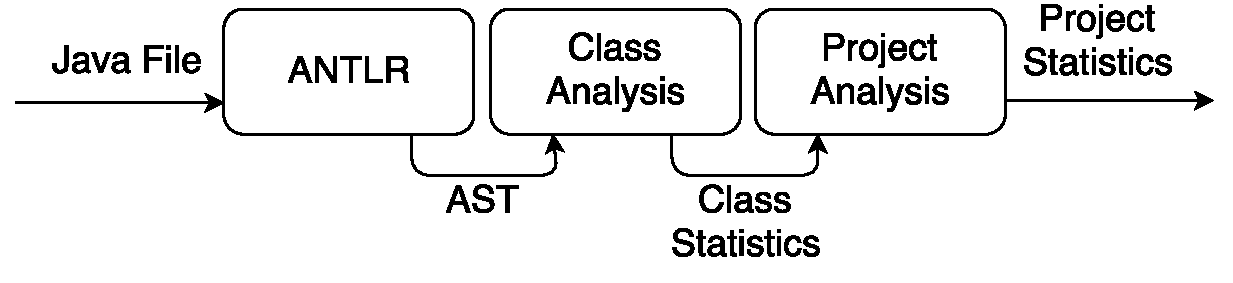
\includegraphics[scale=0.70]{AntlrPipeline.pdf}
\end{center}

\section{\DIFadd{C}\# \DIFadd{Analysis}}
\DIFadd{As with Java, C}\# \DIFadd{was analysed using a lexer and parser generated by loading a C}\# \DIFadd{6 grammar into ANTLR. The analysis for each project in the corpus was performed in three major passes:
}\begin{enumerate}
	\item \DIFadd{Use ANTLR, along with a C}\# \DIFadd{preprocessor grammar, to perform the first stage towards forming a syntax tree. This stage evaluates preprocessor directives in the program to ensure the remaining file can transformed into a well formed syntax tree. Included in this stage is the removal of }\cs{\#region} \DIFadd{tags and conditional directives which exclude and include blocks of source code based on boolean arguments.
	}\item \DIFadd{Use ANTLR, along with a C}\# \DIFadd{program grammar, to create a syntax tree for each C}\# \DIFadd{code file in the corpus and traverse it to find all class declaration subtrees. Collect these class declarations to be explored in later steps.
	}\item \DIFadd{Run a visitor down each class declaration subtree, searching for all the methods and recording their modifiers. A type hierarchy is also established at this step to allow classes to find information about method calls they make which may be dispatched to a method in their superclass.
	}\item \DIFadd{Run another visitor down each class declaration tree and find constructors and check which methods are called against the modifiers found in the previous pass to determine which methods could miss their intended target under a different object initialisation model.
}\end{enumerate}
\DIFadd{The statistics gathered for each file in each project were then aggregated across the corpus to collect information about the corpus as a whole.
}

\section{\DIFadd{JavaScript Analysis}}
\DIFadd{In JavaScript, there are many ways developers make use of classical inheritance patterns despite the lack of native support in the language. This is largely a result of the numerous libraries which offer their own implementation of classical inheritance behaviour. Some examples of these patterns can be found in the following table:
}\begin{center}
	\captionof{table}{JavaScript Patterns}
	\begin{tabular}{|p{5cm}|p{9cm}|}
		\hline
		\multicolumn{2}{|c|}{JavaScript}                                                                                                                                                                  \\ \hline
		\DIFadd{Inheritance 1                  }& \code{var a = function( b )\{    c.call ( this , d );\}}                                                                                      \\ \hline
		\DIFadd{Inheritance 2                  }& \code{function Bar( x , y )\{    Foo.call ( this , x ) ;\}}                                                                                 \\ \hline
		\DIFadd{Inheritance 3                  }& \code{Foo.prototype = object.create ( Bar.prototype )}                                                                                      \\ \hline
		\DIFadd{Inheritance 4 - Node.js        }& \code{var className = defineClass(...)}                                                                                                           \\ \hline
		\DIFadd{Inheritance 5 - Node.js        }& \code{ util.inherits(...)}                                                                                                                         \\ \hline
	\end{tabular}\newline\newline
\end{center}

\DIFadd{As a result of the wide ranging methods of implementing classical inheritance in JavaScript, the effort required to do so accurately is great. Prior work in the field made the JavaScript analysis in this study possible, primarily the existence of tool }\DIFaddend JSClassFinder~\cite{JSClassFinder}. \DIFaddbegin \DIFadd{The JavaScript analysis in this study consisted mainly of a recreation of the JSClassFinder study. JSClassFinder is a tool created by a team of researchers to analyse the extent to which JavaScript developers use classes in their projects.
}

\section{\DIFadd{Lua Analysis}}
\DIFadd{The Lua corpus was analysed with Grep to identify code patterns and keywords associated with class usage. There exists a variety of patterns used to implement object orientation in Lua as described by the Lua-Users Wiki~\mbox{%DIFAUXCMD
\cite{LuaObjectOrientation}
}%DIFAUXCMD
. The analysis in this study attempts to uncover the proportion of the Lua corpus which is making use of object oriented paradigms and, to achieve this, analyses the code of each file to detect the particular patterns found in the object orientation tutorial.
}\DIFaddend \newline

\DIFdelbegin \DIFdel{For the other studied languages, Python, Lua , andScala, quality existing corpora could not be found }\DIFdelend \DIFaddbegin \DIFadd{The first of these patterns is the presence of }\code{[identifier] = setmetatable()} \DIFadd{in a Lua program. The }\code{setmetatable()} \DIFadd{function is the core of all suggested object orientation implementations so the detection of this pattern is vital. Unfortunately, while the use of this function is typically considered necessary for object orientation to exist in a Lua program, the pattern is often encapsulated in a function of a different name which makes the actual extent of object orientation usage more difficult to measure. In response to the practice of encapsulation of these patterns, this study has also included measures of the presence of two function names which are typically used to wrap these classical inheritance behaviours. These are the }\code{class()} \DIFadd{and }\code{new()} \DIFadd{functions}\DIFaddend .
\DIFdelbegin \DIFdel{For each of these languages, the top 25 open source projects were sourced from GitHub's "Trending this month" list for June, 2016. This source was chosen because it provides a group of projects for each language which are in active development as measured by GitHub, and which are easy to access. This helps to ensure that the analysis performed will be as relevant as possible to modern software development.
}\DIFdelend 






 \DIFaddbegin \newpage 
\chapter{\DIFadd{Results}}\label{C:results} 
\DIFaddend \section{Java}
The intent in analysing the Qualitas Corpus of Java code is to determine the extent to which developers are making use of Java's inbuilt language features and what developers are doing to work around these language features. Specifically, a Java developers' usage of class inheritance will represent them conforming to the classical inheritance model encouraged by the Java language. In contrast, instances of code which model call forwarding or call delegation will represent cases where the developer could have expressed themselves more concisely through other object inheritance models where delegation and forwarding are supported natively. The following patterns are used to identify instances of each model of reuse within the Java projects.
\DIFdelbegin %DIFDELCMD < \newline
%DIFDELCMD < %%%
\DIFdelend 

\DIFaddbegin \begin{center}
	\DIFaddend \captionof{table}{Java Patterns}
	\DIFaddbegin \label{JavaPatterns}
	\DIFaddend \begin{tabular}{|p{5cm}|p{9cm}|}
		\hline
		\DIFaddbegin 

		\DIFaddend \multicolumn{2}{|c|}{Java}                                                                   
		\DIFaddbegin 

		\DIFaddend \\ \hline
		\DIFaddbegin 

		\DIFaddend Forwarding                     & \DIFdelbegin \DIFdel{anything name (anything)\{ }\DIFdelend \DIFaddbegin \java{Anything name (anything)\{} \DIFaddend \newline  \hphantom{----}\DIFdelbegin \DIFdel{return identifier}%DIFDELCMD < {[}%%%
\DIFdel{.identifier}%DIFDELCMD < {]}%%%
\DIFdel{*.name(anything);}\DIFdelend \DIFaddbegin \java{return identifier{[}.identifier{]}*.name(anything);} \DIFaddend \newline
		\DIFdelbegin \DIFdel{\}  }\DIFdelend \DIFaddbegin \java{\}}  \DIFaddend \\ 
		\hline
		\DIFaddbegin 

		\DIFaddend Call Delegation                     & \DIFdelbegin \DIFdel{anything name (anything) \{ }\DIFdelend \DIFaddbegin \java{Anything name (anything) \{} \DIFaddend \newline   \hphantom{----}\DIFdelbegin \DIFdel{return identifier}%DIFDELCMD < {[}%%%
\DIFdel{.identifier}%DIFDELCMD < {]}%%%
\DIFdel{*.name(this);}\DIFdelend \DIFaddbegin \java{return identifier{[}.identifier{]}*.name(this);} \DIFaddend \newline \DIFdelbegin \DIFdel{\}  }\DIFdelend \DIFaddbegin \java{\}}		
		\DIFaddend \\ \hline
		\DIFaddbegin 

		\DIFaddend Constructor Delegation & \DIFdelbegin \DIFdel{anything anything = new anything ( this )                                                                                                  }\DIFdelend \DIFaddbegin \java{Anything anything = new anything ( this )}

		\DIFaddend \\ \hline
		\DIFaddbegin 

		\DIFaddend Inheritance                    & \DIFdelbegin \DIFdel{class extends anything                                                                                                                                         }\DIFdelend \DIFaddbegin \java{class extends anything}

		\DIFaddend \\ \hline
	\end{tabular}\newline\newline
\DIFdelbegin %DIFDELCMD < \newline
%DIFDELCMD < %%%
\DIFdelend \DIFaddbegin \end{center}
\DIFaddend 

The presence of two patterns representing delegation is because there are two main ways this behaviour can be represented in Java. The first, call delegation, is where an object passes itself as a parameter to some delegatee and has that delegatee perform some action on its behalf. The second, constructor delegation, is where a delegatee is constructed specifically for the instance of the delegator. This delegatee can then act on that constructor argument when its other methods are called.
\newline\DIFdelbegin %DIFDELCMD < 

%DIFDELCMD < %%%
\DIFdel{Finding occurrences of classical inheritance in Java is as simple as looking for the extends keyword with a "grep" regular expression search. Finding examples of delegation and forwarding is more difficult and requires more information about the syntax tree of the program. To achieve this, each program of the corpus was passed through ANTLR which parses each file according to a Java grammar and constructs an abstract syntax tree which can then be traversed to search for relevant patterns.
}\DIFdelend \newline\DIFdelbegin %DIFDELCMD < 

%DIFDELCMD < %%%
\DIFdel{The process for analysing a Java project follows a pipeline structure where each file is parsed and analysed in isolation. The resulting statistics of each file are then aggregated to form the overall statistics across the projects. This file isolation is important because the syntax trees produced by ANTLR consume large amounts of memory so it is not possible to hold all the Java files for a project in memory simultaneously.
}\DIFdelend \newline

\DIFdelbegin %DIFDELCMD < \captionof{figure}{Java Analysis Pipeline}
%DIFDELCMD < 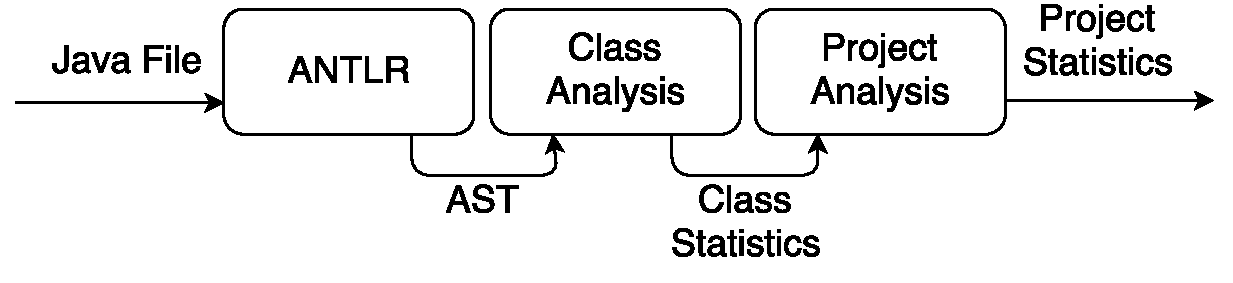
\includegraphics[scale=0.70]{AntlrPipeline.pdf}
%DIFDELCMD < 

%DIFDELCMD < %%%
\DIFdel{The results are then aggregated to }\DIFdelend \DIFaddbegin \DIFadd{The frequency of occurrence of each of the above patterns was calculated and aggregated to }\DIFaddend produce corpus level analysis which can be found in the following table:
\DIFdelbegin %DIFDELCMD < \newline
%DIFDELCMD < %%%
\DIFdelend 

\DIFaddbegin \begin{center}
	\DIFaddend \captionof{table}{Java Analysis Results}
	\DIFaddbegin \label{JavaResults}
	\DIFaddend \begin{tabular}{|l|l|l|l|}
		\hline
		& Count  & \% of classes & \% of extended classes \\ \hline
		\DIFdelbegin \DIFdel{Total classes                                                                                   }\DIFdelend \DIFaddbegin \DIFadd{Projects                                                                                   }\DIFaddend & \DIFdelbegin \DIFdel{116427 }\DIFdelend \DIFaddbegin \DIFadd{112 }\DIFaddend &               &                        \\ \hline
		Classes                                                                                   \DIFdelbegin \DIFdel{extend another class                                                                    }\DIFdelend & \DIFaddbegin \DIFadd{116427 }&               &                        \\ \hline
		\DIFadd{Extending Classes                                                                    }& \DIFaddend 71203  & 61.16\%       &                        \\ \hline
		\DIFdelbegin \DIFdel{Classes are extended by another class                                                           }\DIFdelend \DIFaddbegin \DIFadd{Extended Classes                                                           }\DIFaddend & 20751  & 17.82\%       &                        \\ \hline
		Classes with forwarding                                                                         & 7087   & 6.09\%        &                        \\ \hline
		\begin{tabular}[c]{@{}l@{}}Classes with forwarding\\ that extend another class\end{tabular}     & 3381   & 2.90\%        &                        \\ \hline
		\DIFdelbegin \DIFdel{Classes with downcalls in constructors}\DIFdelend \DIFaddbegin \begin{tabular}[c]{@{}l@{}}\DIFadd{Classes with local}\\ \DIFadd{method calls in constructors}\end{tabular}                                                          \DIFaddend & 16101  & 13.83\%       &                        \\ \hline
		\DIFaddbegin \begin{tabular}[c]{@{}l@{}}\DIFaddend Classes storing this\DIFdelbegin \DIFdel{in constructors                                                            }\DIFdelend \DIFaddbegin \\ \DIFadd{in constructors}\end{tabular}                                                            \DIFaddend & 2392   & 2.05\%        &                        \\ \hline
		\begin{tabular}[c]{@{}l@{}}Classes with \DIFdelbegin \DIFdel{downcalls or}\DIFdelend \DIFaddbegin \DIFadd{local method calls}\DIFaddend \\ \DIFaddbegin \DIFadd{or }\DIFaddend storing this in constructor\end{tabular} & 17099  & 14.69\%       &                        \\ \hline
		\begin{tabular}[c]{@{}l@{}}Extended classes with \DIFaddbegin \DIFadd{local}\DIFaddend \\ \DIFdelbegin \DIFdel{downcalls }\DIFdelend \DIFaddbegin \DIFadd{method calls }\DIFaddend in constructors\end{tabular}       & 1545   & 1.33\%        & 7.45\%                 \\ \hline
		\begin{tabular}[c]{@{}l@{}}Extended classes storing\\ this in constructors\end{tabular}         & 178    & 0.15\%        & 0.86\%                 \\ \hline
		Classes with delegation                                                                         & 5183   & 4.45\%        &                        \\ \hline
	\end{tabular}
\DIFaddbegin \end{center}
\DIFaddend 

\DIFdelbegin \section{\DIFdel{JavaScript}}
%DIFAUXCMD
\addtocounter{section}{-1}%DIFAUXCMD
\DIFdel{In JavaScript, there are many ways developers }\DIFdelend \DIFaddbegin \subsection{\DIFadd{Detecting Delegation}}
\label{DetectingDelegation}
\DIFadd{Due to the imprecise definition of what it means to model delegation in Java, it is expected that some of the results which are returned in the search for these delegation patterns will be false positives. Upon manual inspection of some of the corpus files, some of the patterns which meet the criteria outlined in \ref{JavaPatterns} would not generally be considered to exhibit the true behaviour delegation. An example of this is object self registration where and object registers itself with some other object which will }\DIFaddend make use of \DIFdelbegin \DIFdel{classical inheritance patterns despite the lack of native support in }\DIFdelend the \DIFdelbegin \DIFdel{language}\DIFdelend \DIFaddbegin \DIFadd{registered object in some way. To continue the example of the }\java{Square} \DIFadd{class, an instance of }\java{Square} \DIFadd{could, at construction time,  register itself to a }\java{Canvas} \DIFadd{so that the }\java{Canvas} \DIFadd{can call back to the }\java{Square} \DIFadd{to request details necessary for drawing. The }\java{Square} \DIFadd{class would have a constructor parameter which is a reference to the }\java{Canvas} \DIFadd{object:
}\begin{lstlisting}
\DIFadd{public Square(Canvas canvas)}{
	\DIFadd{canvas.register(this);
}}
\end{lstlisting}
\DIFadd{And a }\java{Square} \DIFadd{could be added to the }\java{Canvas} \DIFadd{as follows:
}\begin{lstlisting}
\DIFadd{void addSquare()}{
	\DIFadd{Square s = new Square(this);
}}
\end{lstlisting}
\DIFadd{This matches the pattern of Constructor Delegation in \ref{JavaPatterns} but , in reality, is modelling a different intent. Because of this, the statistics gathered for delegation should be treated as an upper bound on the actual frequency of occurrence of the behaviour.
}\newline

\subsection{\DIFadd{Unique Class Name Assumption}}
\label{uniqueNames}
\DIFadd{As the Java analysis in this study was performed on source code alone, there are cases of ambiguous class names which would only be disambiguated through full namespace analysis. Because of this, the results are dependent on classes in a package being named uniquely. In cases where this assumption does not hold there is a risk classes being considered to be extended when they are not. More specifically, the question ``Is class A extended by another class" will evaluate to true when any class in the package with the name ``A" is extended by another class. This limits the accuracy of the ``Classes that are extended by another class" metric in table \ref{JavaResults}
}

\section{\DIFadd{C}\#}
\DIFadd{C}\# \DIFadd{is a useful language to investigate because it requires use of the }\cs{virtual} \DIFadd{keyword to enable overriding of any given method, otherwise defaulting to static method dispatch}\DIFaddend . This is \DIFdelbegin \DIFdel{largely a result of the numerous libraries which offer their own implementation of classical inheritance behaviour.
Some examples of these patterns can be found in the following table:
	}%DIFDELCMD < \captionof{table}{JavaScript Patterns}
%DIFDELCMD < \begin{tabular}{|p{5cm}|p{9cm}|}
%DIFDELCMD < 	%%%
\DIFdelend \DIFaddbegin \DIFadd{interesting because it forces the developer to make their intent to override a method explicit, in contrast to Java where virtual dispatch is the default and occurs when the developer has simply omitted the }\java{final} \DIFadd{modifier. This makes it much more clear whether there could potentially be construction issues if we had a different way of initialising objects in place of Uniform Identity. When the }\cs{virtual} \DIFadd{keyword is required, the only method calls which could miss their intended target when used in a constructor are those which are explicitly labelled as }\cs{virtual} \DIFadd{dispatch calls.
}

\begin{center}
	\centering
	\captionof{table}{C\# Analysis Results}
	\label{CsResults}
	\begin{tabular}{|l|l|l|l|}
		\DIFaddend \hline
		\DIFdelbegin %DIFDELCMD < \multicolumn{2}{|c|}{JavaScript}                                                                                                                                                                  %%%
\DIFdelend \DIFaddbegin & \DIFadd{Total  }& \DIFadd{\% of methods }& \DIFadd{\% of classes }\DIFaddend \\ \hline
		\DIFdelbegin \DIFdel{Inheritance 1                  }\DIFdelend \DIFaddbegin \DIFadd{Projects                                                                                                       }\DIFaddend & \DIFdelbegin \DIFdel{var a = function (b ) 
	\{    c .call (this , d ); 
	\}                                                                                      }\DIFdelend \DIFaddbegin \DIFadd{25     }&                    &                    \DIFaddend \\ \hline
		\DIFdelbegin \DIFdel{Inheritance 2                  }\DIFdelend \DIFaddbegin \DIFadd{Classes                                                                                                        }\DIFaddend & \DIFdelbegin \DIFdel{function Bar   (x , y ) 
	\{    Foo .
	call ( this , x ) ;
	\}                                                                                 }\DIFdelend \DIFaddbegin \DIFadd{71539  }&                    &                    \DIFaddend \\ \hline
		\DIFdelbegin \DIFdel{Inheritance 3                  }\DIFdelend \DIFaddbegin \DIFadd{Extending Classes                                                                                              }\DIFaddend & \DIFdelbegin \DIFdel{Foo . prototype = object .
create ( Bar . prototype )                                                                                      }\DIFdelend \DIFaddbegin \DIFadd{19222  }&                    & \DIFadd{26.87\%            }\DIFaddend \\ \hline
		\DIFdelbegin \DIFdel{Inheritance 4 - Node. js        }\DIFdelend \DIFaddbegin \DIFadd{Extended Classes                                                                                              }\DIFaddend & \DIFdelbegin \DIFdel{var className = defineClass(. ..)                                                                                                           }\DIFdelend \DIFaddbegin \DIFadd{9057  }&                    & \DIFadd{12.66\%            }\DIFaddend \\ \hline
		\DIFdelbegin \DIFdel{Inheritance 5 - Node.
js        }\DIFdelend \DIFaddbegin \DIFadd{Methods                                                                                                        }\DIFaddend & \DIFdelbegin \DIFdel{util.
	inherits(.
	..)                                                                                                                         }\DIFdelend \DIFaddbegin \DIFadd{222121 }&                    &                    \DIFaddend \\ \hline
		\DIFaddbegin \DIFadd{Virtual Methods                                                                                                }& \DIFadd{10721  }& \DIFadd{4.83\%             }&                    \\ \hline
		\DIFadd{Override Methods                                                                                               }& \DIFadd{26760  }& \DIFadd{12.05\%            }&                    \\ \hline
		\DIFadd{Delegates                                                                                               }& \DIFadd{738  }&             &                    \\ \hline
		\begin{tabular}[c]{@{}l@{}}\DIFadd{Classes with calls to local}\\ \DIFadd{methods in constructors}\DIFaddend \end{tabular}                  \DIFaddbegin & \DIFadd{1764   }&                    & \DIFadd{2.47\%             }\\ \hline
		\begin{tabular}[c]{@{}l@{}}\DIFadd{Classes with calls to local}\\ \DIFadd{virtual methods in constructors}\end{tabular}          & \DIFadd{48    }&                    & \DIFadd{0.07\%             }\\ \hline
		\begin{tabular}[c]{@{}l@{}}\DIFadd{Classes with calls to local}\\ \DIFadd{override methods in constructors}\end{tabular}         & \DIFadd{55     }&                    & \DIFadd{0.08\%             }\\ \hline
		\begin{tabular}[c]{@{}l@{}}\DIFadd{Classes with calls to local}\\ \DIFadd{abstract methods in constructors}\end{tabular}         & \DIFadd{15     }&                    & \DIFadd{0.02\%             }\\ \hline
		\begin{tabular}[c]{@{}l@{}}\DIFadd{Classes with calls to methods}\\ \DIFadd{that could not be found in constructors}\end{tabular} & \DIFadd{616    }&                    & \DIFadd{0.86\%             }\\ \hline
	\end{tabular}\DIFaddend \newline\newline
\DIFaddbegin \end{center}
\DIFadd{The full C}\# \DIFadd{corpus statistics are broken down for each project and have been included as appendix \ref{A:csProjStats}.
}

\subsection{\DIFadd{Fewer Local Method Calls from Constructors}}
\DIFadd{The first notable difference between the C}\# \DIFadd{results and those for Java is the drastic reduction in the number of calls to local methods from constructors, 2.47\% for C}\# \DIFadd{compared with 13.18\% for Java. There are likely a variety of reasons for this drastic reduction, but of note is that the Microsoft Developer Network Blog strongly discourages this practice~\mbox{%DIFAUXCMD
\cite{NoDowncalls}
}%DIFAUXCMD
, and the widely used Visual Studio extension ReSharper provides IDE warnings against the practice~\mbox{%DIFAUXCMD
\cite{ResharperWarning}
}%DIFAUXCMD
.
}\DIFaddend \newline
\DIFaddbegin 

\subsection{\DIFadd{Virtual Calls from Constructors are Rare}}
\DIFadd{The valuable information gained from the C}\# \DIFadd{analysis which could not be retrieved in the Java analysis is the breakdown of classes with local method calls based on whether those method calls are static or virtual dispatch. The analysis showed that only 0.07\% of all classes contained a call to a method where a virtual, abstract or override declaration was found for that method. These are the method calls which would potentially miss their intended target in a construction environment different from Uniform Identity so the rare occurrence of these cases is valuable information. Across the corpus of 71,162 total classes, only 190 would need to be modified to mitigate potential construction issues under a new object initialisation environment.
}\newline

\subsection{\DIFadd{Methods that could not be found}}
\label{MethodNotFound}
\DIFadd{As with Java, there were some limitations to the accuracy of the analysis performed due to some of the limitations of pure source code analysis. The limits are most obvious in the final row of table \ref{CsResults} where we find that 0.86\% of classes contained a local method call where the destination of that call could not be found. This can occur when the analysis comes across a couple of cases.
}\begin{itemize}
	\item \DIFadd{A constructor contains a non-local method call which is indistinguishable from a local method call without more information. An example of this is the use of C}\#\DIFadd{'s }\cs{using static} \DIFadd{syntax which imports the static functions from another namespace and a allows those functions to be called in a way that looks identical to a local method call. The }\cs{using static} \DIFadd{pattern allows the following code:
	}\begin{lstlisting}[language=cs]
\DIFadd{using System.Console;
class Program : SuperProgram
}{ 
	\DIFadd{static void Main() 
	}{ 
		\DIFadd{Console.WriteLine("Hello world!"); 
	}} 
}
	\end{lstlisting}
	\DIFadd{to be replaced with this implementation:
	}\begin{lstlisting}[language=cs]
\DIFadd{using static System.Console;
class Program : SuperProgram
}{ 
	\DIFadd{static void Main() 
	}{ 
		\DIFadd{WriteLine("Hello world!"); 
	}} 
}
	\end{lstlisting}
	\DIFadd{And without information about the contents of }\cs{System.Console}\DIFadd{, it is not possible to determine that }\cs{WriteLine()} \DIFadd{is a function defined in that namespace.
	}\item \DIFadd{A class extends a class in a pre-compiled library. If a call is made from a constructor to a local virtual or abstract method defined in a pre-compiled superclass then, unless that method has been overridden by the class being analysed, there is no way to know that the method was virtual or abstract.
}\end{itemize}
\DIFadd{While the number of methods which were not found is high at 616, making up 34.9\% of all local method calls in constructors, the remaining 1148 methods which were found were largely without virtual, abstract or override modifiers. Of those 1148 methods only 118, or 10.3\%, had one of these modifiers.
}

\subsection{\DIFadd{Superclasses and Interfaces}}
\label{interfaceNaming}
\DIFadd{In Java, source code alone clearly identifies the distinction between extending a class and implementing an interface. An inheritance relationship is written as
}\begin{lstlisting}[language=java]
\DIFadd{class Square extends Rectangle }{ }
\end{lstlisting}
\DIFadd{whereas indicating that a class implements a given interface is written as
}\begin{lstlisting}[language=java]
\DIFadd{class Square implements Shape }{ }
\end{lstlisting}
\DIFadd{In C}\#\DIFadd{, however, this distinction cannot be determined from source code alone as the syntax elements for both are identical.
}\begin{lstlisting}[language=cs]
\DIFadd{class Square : Rectangle }{ }
\DIFadd{class Square : IShape }{ }
\end{lstlisting}
\DIFadd{To counteract this, the analysis is dependent on the members of the corpus following the C}\# \DIFadd{naming conventions for interfaces as outlined by Microsoft~\mbox{%DIFAUXCMD
\cite{InterfaceNaming}
}%DIFAUXCMD
. This study considers any base type to be an interface when the name of that type is a capital ``I'' character followed by any other uppercase character.
}

\subsection{\DIFadd{Unique Class Name Assumption}}
\DIFadd{The C}\# \DIFadd{results are dependent on the same assumption of unique class names as Java. The reasons for this match those explained in section \ref{uniqueNames}.
}

\subsection{\DIFadd{Distribution of Number of Subclasses}}
\DIFadd{The C}\# \DIFadd{analysis conducted as part of this study resulted in an interesting finding relating to the distribution of the number of subclasses across the classes in the corpus. The analysis revealed that the number of subclasses of extended C}\# \DIFadd{classes approximates a power law distribution, which can be seen in the straight line when the data is rendered onto a log scale. This distribution can be seen in the following chart:
}

\begin{figure}[H]
	\captionof{figure}{Distribution of Number of Subclasses C\# (Log Scale)}
	\label{cSharpDistribution}
	\begin{center}
		
		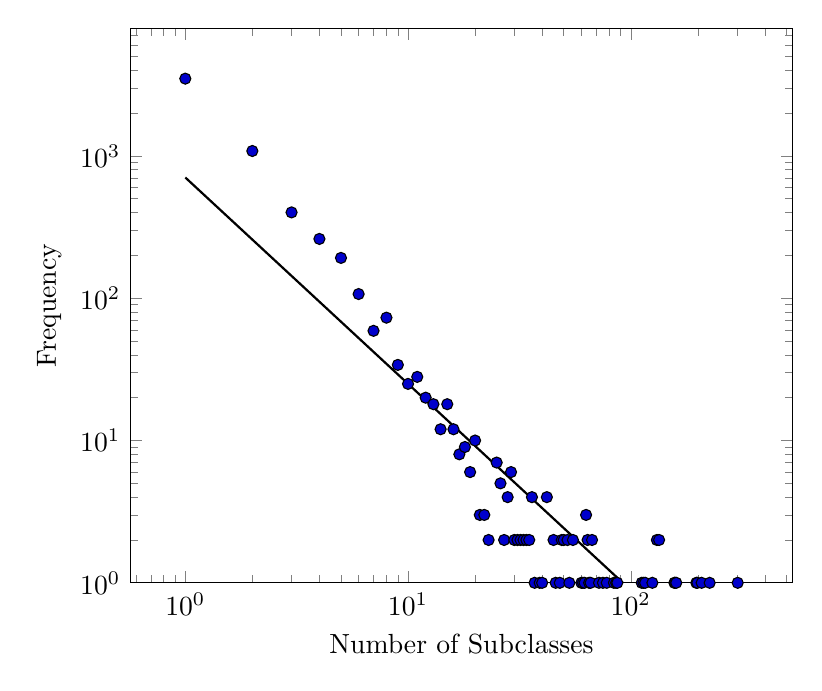
\begin{tikzpicture}
		\begin{axis}[
		xmode = log,
		ymode = log,
		xlabel = Number of Subclasses,
		ylabel = Frequency,
		ymin = 1,
		%title = Distribution of Number of Subclasses C\# (Log Scale)
		]
		\addplot+[only marks, color=black] table {
			1	3492
			2	1083
			3	401
			4	261
			5	192
			6	107
			7	59
			8	73
			9	34
			10	25
			11	28
			12	20
			13	18
			14	12
			15	18
			16	12
			17	8
			18	9
			19	6
			20	10
			21	3
			22	3
			23	2
			25	7
			26	5
			27	2
			28	4
			29	6
			30	2
			31	2
			32	2
			33	2
			34	2
			35	2
			36	4
			37	1
			39	1
			40	1
			42	4
			45	2
			46	1
			48	1
			49	2
			50	2
			52	2
			53	1
			55	2
			60	1
			61	1
			62	1
			63	3
			64	2
			65	1
			66	1
			67	2
			72	1
			75	1
			78	1
			84	1
			86	1
			87	1
			112	1
			114	1
			116	1
			125	1
			131	2
			134	2
			157	1
			158	1
			160	1
			197	1
			199	1
			208	1
			226	1
			302	1
		};
		
		\addplot [thick, black] table[y={create col/linear regression}]{
			1	3492
			2	1083
			3	401
			4	261
			5	192
			6	107
			7	59
			8	73
			9	34
			10	25
			11	28
			12	20
			13	18
			14	12
			15	18
			16	12
			17	8
			18	9
			19	6
			20	10
			21	3
			22	3
			23	2
			25	7
			26	5
			27	2
			28	4
			29	6
			30	2
			31	2
			32	2
			33	2
			34	2
			35	2
			36	4
			37	1
			39	1
			40	1
			42	4
			45	2
			46	1
			48	1
			49	2
			50	2
			52	2
			53	1
			55	2
			60	1
			61	1
			62	1
			63	3
			64	2
			65	1
			66	1
			67	2
			72	1
			75	1
			78	1
			84	1
			86	1
			87	1
			112	1
			114	1
			116	1
			125	1
			131	2
			134	2
			157	1
			158	1
			160	1
			197	1
			199	1
			208	1
			226	1
			302	1
		};
		
		\end{axis}
		\end{tikzpicture}
	\end{center}
\end{figure}

\DIFadd{The C}\# \DIFadd{subclassing distribution in \ref{cSharpDistribution} matches the distribution found through the investigation in }\textit{\DIFadd{Understanding the Shape of Java Software}}\DIFadd{~\mbox{%DIFAUXCMD
\cite{ShapeOfJava}
}%DIFAUXCMD
. The distribution found in the analysis of the Java corpus can be found in figure \ref{JavaSubclassDistribution}.
}

\begin{center}
	\captionof{figure}{Distribution of Number of Subclasses in Java (Log Scale)~\mbox{%DIFAUXCMD
\cite{ShapeOfJava}
}%DIFAUXCMD
}
	\label{JavaSubclassDistribution}
	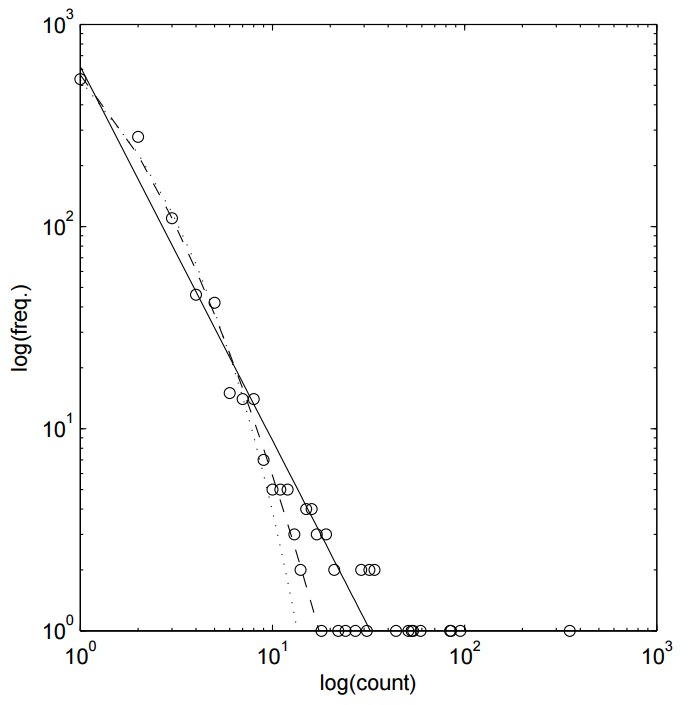
\includegraphics[scale=0.50]{SubclassDistributionJava.png}
\end{center}

\subsection{\DIFadd{Outliers}}
\DIFadd{An interesting outlier file was found during the C}\# \DIFadd{analysis carried out in this study. A file titled }\code{T\_1247520.cs} \DIFadd{is defined in the Roslyn compiler project and is used in testing scenarios. This file contains 10,020 class definitions, each with no superclass, no subclasses, and no method or constructor definitions. The file is found in a }\code{Test} \DIFadd{directory so the assumption is that it is used as a compiler stress test. This file has been left in the corpus for the results found table \ref{CsResults} because I believe removing it would be making the disingenuous claim that all the file in the other corpora had been investigated to ensure they had no similar outliers. Despite this, it is interesting to see the changes to results when these class definitions are removed, thereby reducing the number of classes found by 10,020 but leaving the remaining counts unchanged.
}\begin{itemize}
	\item \DIFadd{The percentage of classes which extend another class increases from 26.87\% to 31.24\%.
	}\item \DIFadd{The percentage of classes which are extended by another class increases from 12.66\% to 14.72\%.
	}\item \DIFadd{The percentage of classes which make calls from local methods from a constructor increases from 2.47\% to 2.87\%.
	}\item \DIFadd{The percentage of classes with calls to local virtual, override, and abstract methods from their constructors increases proportionately with the change in all calls to local methods from constructors.
}\end{itemize}

\section{\DIFadd{JavaScript}}
\DIFaddend The JavaScript analysis in this study makes extensive use of the prior work in developing the JSClassFinder application~\cite{JSClassFinder}. The aim here is to find the cases where JavaScript developers are choosing not to use the native delegation support of the language and are instead modelling their programs with classical inheritance structures. The important factor here is the Class Usage Ratio (CUR) of a JavaScript project as defined in \textit{Does JavaScript Software Embrace Classes?~\cite{JSClassFinder}}. Across a corpus of 50 JavaScript projects, the JSClassFinder returns interesting results about the prevalence of class usage in the language.
\begin{enumerate}
	\item The median CUR across the corpus was 0.15
	\item The upper quartile CUR across the corpus was 0.36
	\item The lower quartile CUR across the corpus was 0.005, which was heavily impacted by 13 systems which had a CUR of zero
\end{enumerate}

\DIFdelbegin \section{\DIFdel{Timeline}}
%DIFAUXCMD
\addtocounter{section}{-1}%DIFAUXCMD
\DIFdel{The corpora for each of the remaining languages have been collected and the next stage is to analyse each to gather statistics which can be compared to those gathered for Java and JavaScript. The aim is to have a paper ready for the upcoming ECOOP paper submission deadline.
}\DIFdelend \DIFaddbegin \DIFadd{This indicates that, in the median project in the JavaScript corpus, 15\% of all functions are modelling some form of class or method behaviour. A value of this magnitude shows that the use of classical inheritance in JavaScript is highly prevalent despite the language's lack of native support for its implementation.
}

\section{\DIFadd{Lua}}
\DIFadd{Table \ref{LuaResults} shows a variety of patterns often representative of class usage and the percentage of files in the corpus which exhibit one or more of those patterns.}\DIFaddend \newline
\DIFdelbegin %DIFDELCMD < \captionof{figure}{Project Timeline}
%DIFDELCMD < \begin{ganttchart}[
%DIFDELCMD < 	hgrid,
%DIFDELCMD < 	vgrid={*{6}{draw=none},dotted},
%DIFDELCMD < 	x unit=0.87mm,
%DIFDELCMD < 	group peaks tip position=0,
%DIFDELCMD < 	group peaks height=.2,
%DIFDELCMD < 	group peaks width=2,
%DIFDELCMD < 	time slot format=isodate
%DIFDELCMD < 	]{2016-07-08}{2016-11-11}
%DIFDELCMD < 	%%%
\DIFdel{14
	}%DIFDELCMD < \gantttitlecalendar{month=shortname} %%%
\DIFdelend \DIFaddbegin 

\DIFadd{Often functions called }\code{class()} \DIFadd{will be created to encapsulate the }\java{setmetatable()} \DIFadd{logic which is used to create classes. It is also common to declare functions with the name }\code{new()} \DIFadd{for use as constructors.
}

\begin{center}
	\captionof{table}{Lua Analysis Results}
	\label{LuaResults}
	\begin{tabular}{|l|l|l|l|}
		\hline
		\DIFadd{Pattern                 }& \DIFadd{Test               }& \DIFadd{Result }& \DIFadd{Percentage }\DIFaddend \\ \DIFdelbegin %DIFDELCMD < \ganttgroup{Language Analysis}{2016-07-08}{2016-09-01}%%%
\DIFdelend \DIFaddbegin \hline
		\DIFadd{= setmetatable(        }&                    &        &            \DIFaddend \\ \DIFdelbegin %DIFDELCMD < \ganttbar{JavaScript}{2016-07-08}{2016-07-21}%%%
\DIFdelend \DIFaddbegin \hline
		& \DIFadd{Total matches      }& \DIFadd{135    }&            \DIFaddend \\ \DIFdelbegin %DIFDELCMD < \ganttbar{Python}{2016-07-22}{2016-08-04}%%%
\DIFdelend \DIFaddbegin \hline
		& \DIFadd{Files with matches }& \DIFadd{74     }& \DIFadd{2.67\%     }\DIFaddend \\ \DIFdelbegin %DIFDELCMD < \ganttbar{Scala}{2016-08-05}{2016-08-18}%%%
\DIFdelend \DIFaddbegin \hline
		\DIFadd{class(                  }&                    &        &            \DIFaddend \\ \DIFdelbegin %DIFDELCMD < \ganttbar{Lua}{2016-08-19}{2016-09-01} %%%
\DIFdelend \DIFaddbegin \hline
		& \DIFadd{Total matches      }& \DIFadd{487    }&            \DIFaddend \\ \DIFdelbegin %DIFDELCMD < \ganttgroup{Collective Analysis}{2016-09-02}{2016-10-13}%%%
\DIFdelend \DIFaddbegin \hline
		& \DIFadd{Files with matches }& \DIFadd{380    }& \DIFadd{13.69\%    }\DIFaddend \\ \DIFdelbegin %DIFDELCMD < \ganttbar{Comparing Analyses}{2016-09-02}{2016-09-23}%%%
\DIFdelend \DIFaddbegin \hline
		\DIFadd{function something.new( }&                    &        &            \DIFaddend \\ \DIFdelbegin %DIFDELCMD < \ganttbar{Final Report}{2016-09-02}{2016-10-13}%%%
\DIFdelend \DIFaddbegin \hline
		& \DIFadd{Total matches      }& \DIFadd{31     }&            \DIFaddend \\ \DIFdelbegin %DIFDELCMD < \ganttgroup{Presentation}{2016-10-14}{2016-11-11}%%%
\DIFdelend \DIFaddbegin \hline
		& \DIFadd{Files with matches }& \DIFadd{30     }& \DIFadd{1.08\%     }\DIFaddend \\ \DIFdelbegin %DIFDELCMD < \ganttbar{Creating Presentation}{2016-10-14}{2016-10-27}%%%
\DIFdelend \DIFaddbegin \hline
		\DIFadd{Union of all three      }&                    &        &            \DIFaddend \\ \DIFdelbegin %DIFDELCMD < \ganttbar{Rehearsing Presentation}{2016-10-28}{2016-11-11}
%DIFDELCMD < \end{ganttchart} %%%
\DIFdelend \DIFaddbegin \hline
		& \DIFadd{Total matches      }& \DIFadd{653    }&            \\ \hline
		& \DIFadd{Files with matches }& \DIFadd{473    }& \DIFadd{17.04\%    }\\ \hline
	\end{tabular}
	\newline
	\newline
\end{center}

\DIFadd{These results show that the proportion of Lua developers making use of classical inheritance patterns is high, with around 17\% of all Lua files in the examined corpus presenting class-like behaviour of some kind.
}


\section{\DIFadd{Evaluation}}
\DIFadd{The accuracy of the results of this study can be measured in terms of false positives against true positives and false negatives against true negatives. These can each be measured in different ways, but the process of testing for false positives is easier and more reliable than testing false negatives.
}\newline

\DIFadd{False positives occur when the algorithms used to detect patterns in the corpora claim to have found an instance of that pattern, but the code does not match the definition exactly. Detecting false positives in the data can be achieved by investigating the results returned as matches against the patterns in the analysis to determine whether the are, in fact, exhibiting the behaviour for which the pattern is searching. In cases where the algorithms used to detect the patterns could be modified to ignore the false positives, the were, but in cases where the algorithms could not be easily fixed, this has been explained. Examples of these are as follows.
}\begin{itemize}
	\item \DIFadd{False positives may be returned for extendedness when the interface naming assumption explained in section \ref{interfaceNaming} fails and an interface is named in a way that makes in indistinguishable from a class.
	}\item \DIFadd{False positives may be returned for extendedness when the unique class name assumption explained in section \ref{uniqueNames} fails as classes may be considered extended when another class of the identical name is extended.
	}\item \DIFadd{False positives for delegation can occur when developers use code patterns which look identical to those of delegation but are modelling different intents. This is explained in more detail in section \ref{DetectingDelegation}.
	}\newline
\end{itemize} 

\DIFadd{False negatives occur when the algorithms overlook code segments in the corpora which fulfil the criteria to be defined as an instance of the patterns under investigation. Examples of these cases are as follows.
}\begin{itemize}
	\item \DIFadd{There is room for false negatives in the C}\# \DIFadd{statistics on calls to local methods from constructors. The accuracy of this data is limited by the problem of inaccessible external code and the }\cs{using static} \DIFadd{pattern as explained in section \ref{MethodNotFound}. This is reflected in the final row of the table which measures the number of calls from constructors where the receiver of the call either could not be found or was another form of method call which was indistinguishable from a local method call.
	}\item \DIFadd{False negatives for subclassing in C}\# \DIFadd{can exist if a class is defined with a name which fulfils the requirements of the naming convention for interfaces as discussed in section \ref{interfaceNaming}.
}\end{itemize}









%DIF >  \newpage \chapter{Discussion}\label{C:discussion}
\DIFadd{TODO - Possibly merged with results }\DIFaddend \newpage 
 \newpage \chapter{Conclusions}\label{C:con}
Some conclusions can be drawn from the data gathered \DIFdelbegin \DIFdel{thus far. This data covers the analyses of Java and JavaScript corpus data. }\DIFdelend \DIFaddbegin \DIFadd{in this study. }\DIFaddend It was found that there was a reasonable amount of crossover between the native support offered by each language and the patterns used by developers:
\begin{itemize}
	\item In Java, where classical inheritance is natively supported, 6.09\% of classes used forwarding patterns and 4.45\% of classes used delegation patterns.
	\item In JavaScript, where delegation is natively supported, \DIFdelbegin \DIFdel{36}\DIFdelend \DIFaddbegin \DIFadd{15}\DIFaddend \% of the functions in the median project were used to emulate class or method behaviour.
	\DIFaddbegin \item \DIFadd{In Lua, where delegation is natively supported, 17.04\% of all files contained patterns indicative of class behaviour.
}\DIFaddend \end{itemize}
From these numbers, it appears developers are more \DIFdelbegin \DIFdel{wiling to use }\DIFdelend \DIFaddbegin \DIFadd{willing to use classical }\DIFaddend inheritance structures, thus ignoring native delegation. Further research on other languages will help to clarify this claim. \DIFaddbegin \DIFadd{It is difficult to determine whether this is because classical inheritance is necessary for aspects of the projects or if its use is simply more common because developers find it more comfortable.
}\newline

\DIFadd{The further findings of this study involve a measurement of the difficulty involved in reimplementing projects built for classical inheritance into a language built for delegation. The main issues for this reimplementation are constructor patterns which are dependent on uniform identity. It was found, through the Java corpus analysis, that 13.83\% of classes made local calls from constructors and 2.05\% stored }\java{this} \DIFadd{from a constructor. Through the C}\# \DIFadd{corpus analysis, it was found that only around 10.3\% of calls to local methods from constructors are dispatched virtually at runtime. In C}\#\DIFadd{, only 0.17\% of classes contained a call from a constructor to a non-static method. }\DIFaddend \newpage 
 \DIFaddbegin \newpage \chapter{\DIFadd{Limitations and Future Work}}\label{C:future}
\DIFaddend 

\DIFaddbegin \section{\DIFadd{Limitations}}
\DIFadd{There are some innate limitations to the data which can be gathered through static analysis of source code as carried out in this study. These limitations are largely a result of two factors. First, the inability to analyse code which is used by, but is not part of, the project; second, the disconnect between how often particular patterns are written (static frequency) and how often they are actually used during execution (dynamic frequency).
}

\subsection{\DIFadd{Inaccessible External Code}}
\label{InaccessibleCode}
\DIFadd{When only analysing source files, it is not possible to collect information about pre-compiled units which are used by those source files at runtime~\mbox{%DIFAUXCMD
\cite{StaticAnalysisLimits}
}%DIFAUXCMD
. An example of where this can limit the effectiveness of the analysis in this study is the absence of information about calls dispatched to a superclass when that superclass is defined in a pre-compiled library. If a source code file defines a class }\code{A} \DIFadd{which extends a class }\code{B} \DIFadd{where }\code{B} \DIFadd{is defined in a library with precompiled or otherwise inaccessible source code, we cannot see the details of the methods defined in }\code{B}\DIFadd{. This becomes an }\textsl{}\DIFadd{issue because it is no longer possible to determine whether a local call in }\code{A} \DIFadd{which targets a method defined on }\code{B} \DIFadd{will be dispatched statically or virtually because we cannot see the method declaration. This could cause unforeseen changes to the behaviour of the methods on }\code{A} \DIFadd{if another class }\code{C} \DIFadd{were to extend }\code{A} \DIFadd{and override methods from }\code{B} \DIFadd{which we were previously unaware were virtually dispatched calls.
}

\subsection{\DIFadd{Static vs. Dynamic Frequency}}
\DIFadd{It is generally not possible to determine whether any particular class or method is actually used in the execution of a program, or to determine which classes and methods are used more frequently at runtime than others. For example, we might prefer give a different weighting in our analyses to the patterns used in unit test files on the assumption that these are typically written with the expectation that they will rarely need to undergo structural changes after they are written. The are also expected to be executed less frequently than other core functionality in general operation of the program.
}

\subsection{\DIFadd{Technical Limitations}}
\DIFadd{The Mono project in the C}\# \DIFadd{corpus had to be modified to allow the project to be analysed successfully due to technical constraints. As the Mono project sets out to provide an open source implementation of the necessary components of a C}\# \DIFadd{compiler, it contained a copy of the entire .NET core library. This library was over 500MB in size so, after conversion to syntax trees through ANTLR, could not be reasonably analysed within 16GB of ram. For this reason, and because none of the other projects in this study or in \mbox{%DIFAUXCMD
\cite{QualitasCorpus}
}%DIFAUXCMD
included copies of the source of their libraries, the .NET core library was removed from the Mono project. Every project across the corpora studied will have some dependency on a library, even if it is just the languages core libraries, so removing a copy of these libraries from Mono will ensure its comparability with the rest of the analysed data.
}

\subsection{\DIFadd{Incomplete Source Files}}
\DIFadd{There were cases of files in the JavaScript corpus which could not be parsed in isolation to form a valid syntax tree because they were not syntactically valid source. One example of this was a file which consisted of the majority of a valid JavaScript file but stopped short of the end, with a few other files in the same directory offering several different options for the final part of the code. The assumption here was that the files would be opened and appended at runtime but this was not possible to replicate in a study which operates on source code alone. This study ignored files which could not be compiled on their own, but it is possible that data was lost by ignoring files which expect to be concatenated to create valid programs.
}

\section{\DIFadd{Future Work}}
\DIFadd{There are a few other methods of software analysis which can work around the issues outlined above to provide a clearer understanding of a software project than analysis based solely on source code.
}

\subsection{\DIFadd{Analysis of Compiled Units}}
\DIFadd{Analysis of compiled units would help to mitigate the issues explained in section \ref{InaccessibleCode} where precompiled libraries are inaccessable to the analysis. Java and C}\# \DIFadd{both provide intermediate representations in the form of bytecode languages. For Java this is the Java Bytecode Language~\mbox{%DIFAUXCMD
\cite{JVMSpec}
}%DIFAUXCMD
and for C}\# \DIFadd{this is Microsoft's Common Intermediate Language~\mbox{%DIFAUXCMD
\cite{CommonIntermediateLanguage}
}%DIFAUXCMD
. An analysis of these intermediate representations would be useful because they both offer varied instructions for method calls depending on whether the call is virtually or statically dispatched. This helps to overcome the limitation of being unaware of how a call will be dispatched when analysing source code only.
}

\subsection{\DIFadd{Analysis of Dynamic Frequency}}
\DIFadd{Analysing a program at runtime could provide useful information about how often particular patterns are used, as opposed to how often they are written. In JavaScript and Lua, a simple way to achieve this would be to modify commonly used libraries associated with classical inheritance implementations to add counters which record how often classes are created, modified or instantiated. In Java, a program called JVM Monitor~\mbox{%DIFAUXCMD
\cite{JVMMonitor}
}%DIFAUXCMD
could be used to determine the invocation counts of methods which are of interest. This would allow code which is core to the functionality of the program to be weighted more heavily and code which is run relatively infrequently to be weighted more lightly.
}

\subsection{\DIFadd{Measuring Precision and Recall}}
\DIFadd{As with the study }\textit{\DIFadd{Does JavaScript Software Embrace Classes?}} \DIFadd{which describes the creation of the JSClassFinder tool~\mbox{%DIFAUXCMD
\cite{JSClassFinder}
}%DIFAUXCMD
, I had difficulty accurately measuring the exact precision and recall values for my analyses. This is largely because of the difficult in differentiating between a developer's intent and the patterns they use in their code. Even when manually inspecting files and analysis results, it is often not possible to determine whether the result of the analysis is truly indicative of the developer's intent. For this reason, it is only possible to approximate the values of precision and recall based on some assumptions about whether certain patterns are, in fact, representative of the behaviours under analysis. Despite this, having ranges of these precision and recall values could help to improve confidence in the research.
}



 \newpage 

\DIFaddend %%%%%%%%%%%%%%%%%%%%%%%%%%%%%%%%%%%%%%%%%%%%%%%%%%%%%%%
\backmatter

%%%%%%%%%%%%%%%%%%%%%%%%%%%%%%%%%%%%%%%%%%%%%%%%%%%%%%%

%\bibliographystyle{ieeetr}
\bibliographystyle{acm}
\bibliography{sample}

%DIF < \begin{appendices}
\DIFaddbegin \begin{appendices}
\chapter{\DIFadd{C}\# \DIFadd{Analysis by Project}}
\label{A:csProjStats} 
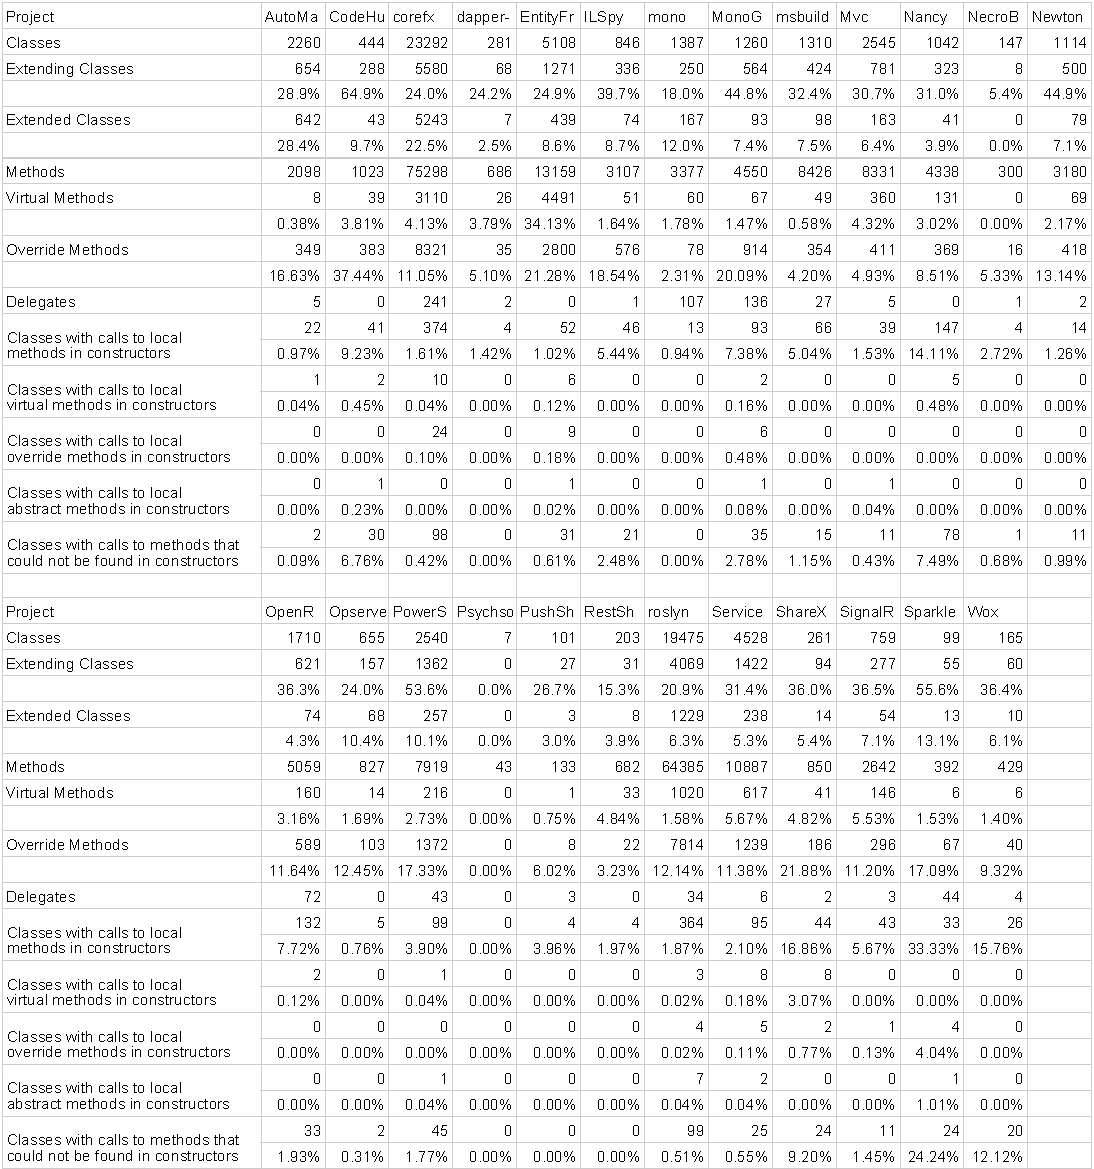
\includepdf[pages=-, scale=0.9]{ProjectSpecificAnalysis.pdf}
\DIFaddend %\chapter{Project Proposal Slides}
%This appendix includes the presentation slides from the proposal of this project.
%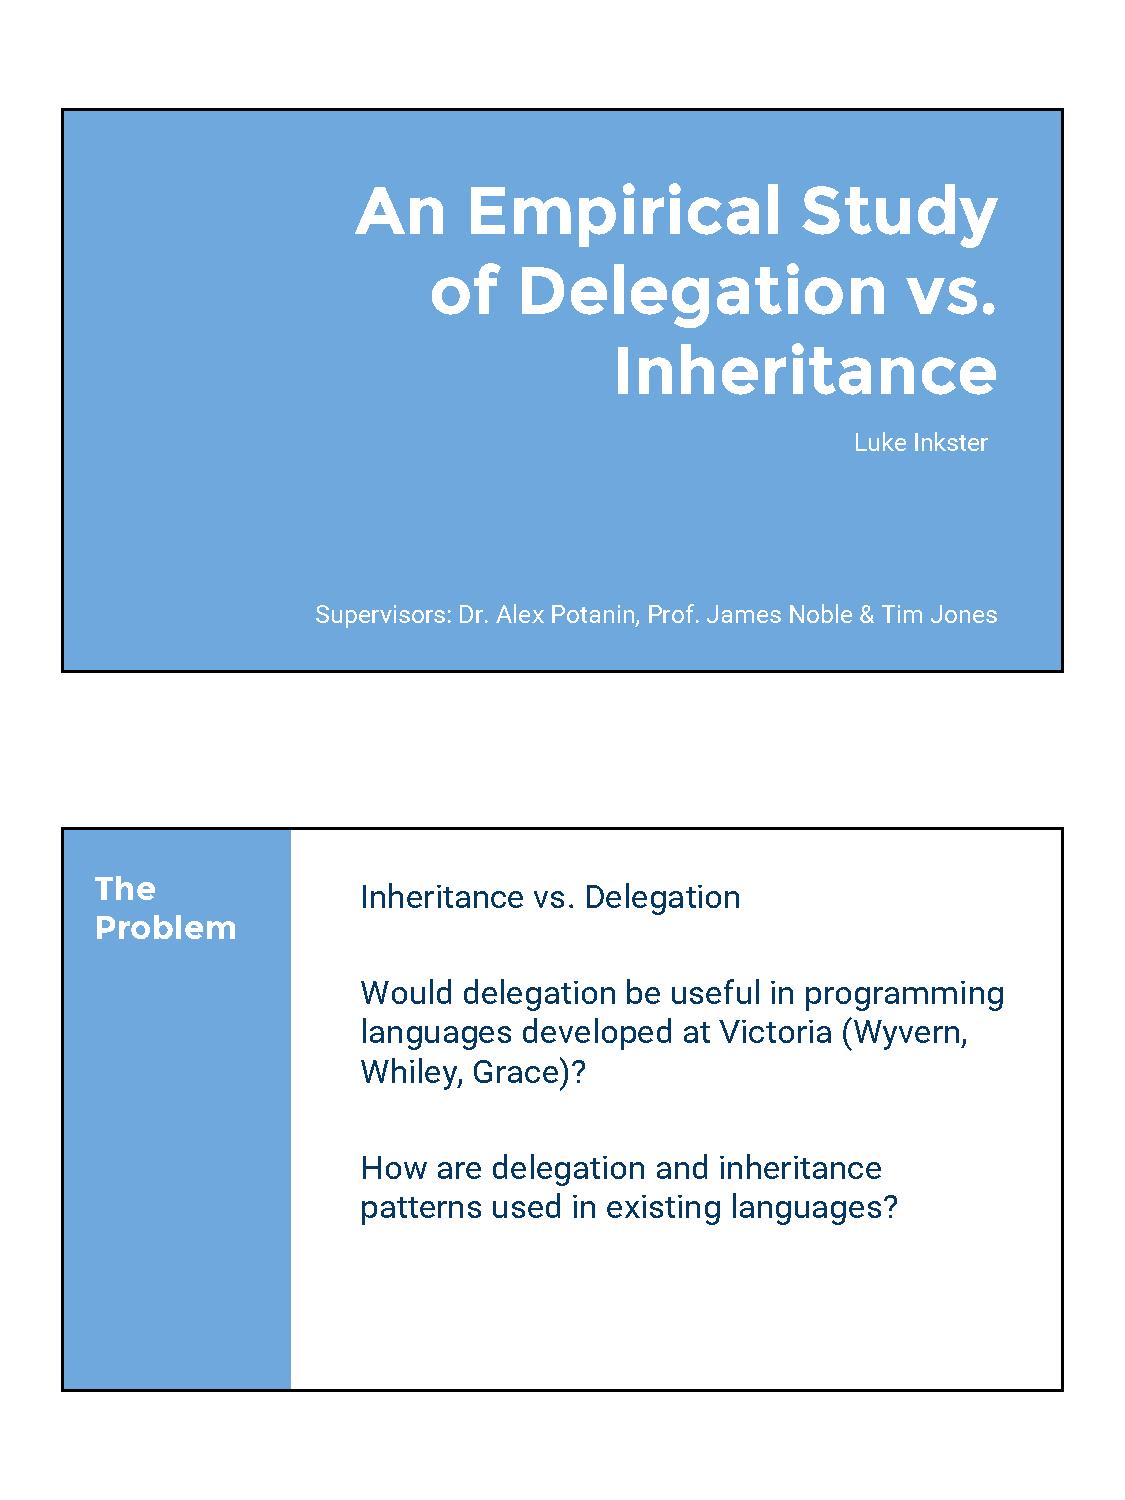
\includepdf[pages=-]{ProposalSlides.pdf}
%DIF < \end{appendices}
\DIFaddbegin \end{appendices}
\DIFaddend 

\end{document}
